\subsection{Unfolding procedures}

\subsubsection{Introduction}
\label{sec:UnfoldIntro}

Unfolding is the process of removing detector effects from data in order to infer the properties of particle-level spectra (see~\cite{Cowan:2002in,Blobel:2203257,doi:10.1002/9783527653416.ch6,Balasubramanian:2019itp} for reviews).  In other fields, this is often called \textit{deconvolution}, since one can think of detector effects as the convolution of a noise function with the spectrum of interest.  Unfolding needs to correct for many effects:

\begin{enumerate}[label={(\arabic*)}]
\item Acceptance and efficiency: particles produced may not be measured.
\item Detector noise: particles measured may not be from real particles, at least not the desired particles (e.g. fakes) within a fiducial volume (migrating into acceptance).
\item Background processes: if one wants to measure the differential cross section of a particular process, then you may want to subtract the contributions from background processes.
\item Combinatorics: if there are $n$ particles and you want to measure the properties of a particular order (e.g. leading $p_T$), the detector effects can change the order.
\item Detector distortions: the detector response introduces bias and resolution effects.
\end{enumerate}

A well-structured measurement will be dominated by (5).  It is possible to setup a measurement so that (4) is not relevant (e.g. operating at the level of events as sets instead of using individual objects).  By using a pure (e.g. $Z$+jets) or inclusive (e.g. dijets) event selection, (3) can be made irrelevant.  It is also possible to mitigate (1) and (2) by performing the unfolding in a bigger phase space than is eventually used for the final measurement.  In our case, we will also reduce these effects by using the highly efficient $Z$ to select events and then using (mostly) the hadronic recoil for the measurement.

Corrections are derived using simulations, by creating a match between particle-level events and detector-level events.  Until now, all measurements in high energy physics have been performed using binned data.   In this case, detector effects can be modeled by a set of linear equations:
\begin{align}
\label{eq:foldingequation}
\left(\textbf{R}\cdot (\textbf{t}\odot \textbf{c})\right)\odot 1/\textbf{f}+\textbf{b}=\textbf{d}\,,
\end{align}
where bold letters denote vectors or matrices, $\cdot$ is the usual matrix product, $\odot$ is the Hadamard (component-wise) product, and the division is defined component-wise\footnote{An equivalent way to write Eq.~\ref{eq:foldingequation} is $\left(\sum_{i}R_{ij}\,t_i\,c_i\right)/f_j+b_j=d_j$, where $i$ and $j$ are indices for the reconstructed and particle level bins, respectively.}. The symbol $\textbf{t}$ is the particle-level distribution, $\textbf{d}$ is the detector-level distribution, $\textbf{b}$ is the background detector-level distribution, and $\textbf{R}$ is the response matrix.  The correction factors $\textbf{c}$ represent the fraction of particle-level events that also pass the detector-level selection and the fake factors $\textbf{f}$ represent the fraction of detector-level events that have a corresponding particle-level event that passes the selection.  The solution to Eq.~\ref{eq:foldingequation} is given by
\begin{align}
\label{eq:unfolding}
\textbf{t}_\text{measured} = \textbf{R}^{-1}\left( (\textbf{d}-\textbf{b})\odot \textbf{f}\right)\odot 1/\textbf{c}.
\end{align}
Many of the of the common unfolding methods follow the form in Eq.~\ref{eq:unfolding}.
Uncertainties on the measurement are obtained using uncertainty propagation. In particular, the unfolding uncertainties are evaluated by varying the response matrix term $\mathbf{R}^{-1}$, which typically is done coherently with the $\mathbf{f}$ and $\mathbf{c}$ terms (e.g.\ by switching MC generator or propagating an experimental or theoretical systematic that affect the event kinematics).
%but vary in their estimation of $\textbf{R}^{-1}$.
For a variety of reasons, it is advantageous to not directly invert the response matrix.  In particular, \textbf{R} may not be invertible because it is singular or not even a square matrix.  The simple matrix inverse is also susceptible to oscillations from significant off-diagonal components.

One of the most widely used unfolding methods is the Iterative Bayesian Unfolding (IBU) technique\footnote{In other fields, this is called Lucy-Richardson deconvolution~\cite{1974AJ.....79..745L,Richardson:72}.}.   For simplicity, assume that $\textbf{b}=\textbf{0}$ and $\textbf{f}=\textbf{c}=\textbf{1}$.  When this is not the case, these are corrected for in the binned case as done in Eq.~\ref{eq:unfolding}.   The IBU method then proceeds as follows:
\begin{align}
t_i^{(n)}&=\sum_j \Pr(t_i|d_j) d_j \\
&=\sum_j \frac{\Pr(d_j|t_i)\Pr^{(n)}(t_i)}{\sum_i \Pr(d_j|t_i)\Pr^{(n)}(t_i)} d_j \\
&=\sum_j \frac{R_{ji}\Pr^{(n)}(t_i)}{\sum_i R_{ji}\Pr^{(n)}(t_i)} d_j.
\end{align}
%
Typically, one choses the prior $\Pr^{(n)}(t_i)=t_i^{(n-1)}$ and $\Pr^{(0)}(t_i)=t_i$ (from simulation), assuming $\textbf{t}$ is normalized.  It has been shown that as $n\rightarrow\infty$, the IBU estimate approaches the maximum likelihood estimator~\cite{shepp1982maximum}.  Typically, $n\sim 3$ as a form of regularization to balance amplifying statistical fluctuations with mitigating systematic uncertainties from the prior dependence.

\subsubsection{OmniFold}
\label{subsec:omnifold}

IBU and other standard unfolding methods face three challenges.  First, they require the data to be binned.  This binning must be chosen ahead of time and is often chosen manually.  Second, only a small number of observables (or a small number of bins for a given number of observables) can be unfolded simultaneously in order to keep the total number of bins to a manageable level.  Finally, the matrix $\textbf{R}$ only depends on the unfolded features and not on any other auxiliary features that may be useful for determining the detector response.  Even though the inputs to the unfolding may be calibrated, if the detector response depends on additional features, the result will be suboptimal and potentially biased.

OmniFold is an approach that addresses all three of the above challenges by using neural networks.  Like IBU, OmniFold is an iterative method.  Furthermore, OmniFold is a natural generalization of IBU in the sense that when the OmniFold method is applied to binned data, it reproduces IBU at each iteration.
As the Omnifold method is unbinned, it works directly with events and we will use $\vec{x}_i$ as the particle-level properties of event $i$, and $\vec{x}_{\mathrm{reco},i}$ would be the corresponding detector-level quantities ($i$ is no longer a bin index as in previous equations).  The properties could be a fixed set of observables or they could be a variable-length set of particles, each with their own properties.  OmniFold can handle any of these cases (with a suitably chosen neural network architecture).
The OmniFold method proceeds as follows:

\begin{description}
\item Iterate:
  \begin{enumerate}[label={(\arabic*)}]
    \item Determine a reweighting function $\omega(\vec{x}_\mathrm{reco})$ that adjusts the detector-level simulation (`MC Reco') to match data (`Data Reco').
    \item Propagate the weights from (1) to the particle-level simulation (`MC Truth'), and determine a new reweighting function $\nu(\vec{x})$ that replicates this reweighing based on particle-level quantities $\vec{x}$. The particle level weights $\nu(\vec{x})$ are next propagated to detector-level.
 \end{enumerate}
\end{description}
%
The final result after $n$ iterations is a function $\nu(\vec{x})$ that provides weights to a particle-level MC sample such that will become ``unfolded data'' for any observable constructed from the event features $\vec{x}$.

As an algorithm, the OmniFold procedure does not require neural networks; however, these tools are well-suited to be the reweighting functions described above (more on this below).  Step (2) of the OmniFold algorithm is important because the weights from (1) are not a function of the particle-level phase space.  In particular, two events in the same particle-level phase space can be mapped to different detector-level events.  However, to be a proper unfolding, we require that two events with the same particle-level phase space have the same weight.  This is achieved with Step (2).

The OmniFold procedure is illustrated schematically in Fig.~\ref{fig:omnifoldschematic}.  The detector-level weights at a given step are represented by the symbol $\omega_n$ while the particle-level weights are represented by the symbol $\nu_n$.  Note that for Step (2), we could reweight from the original particle-level simulation to the weighted simulation or from the weights derived at the previous step to weights from (1).  Both achieve the same results, but there may be advantages to learning an incremental reweighting (as in Fig.~\ref{fig:omnifoldschematic}) since each step is a correction on the previous step.

As mentioned, the output of the OmniFold method is a set of events with weights.  One can then construct any observables from the features used in the unfolding, and from those features, one can construct histograms using whatever binning is desired.

\begin{figure}[h!]
\centering
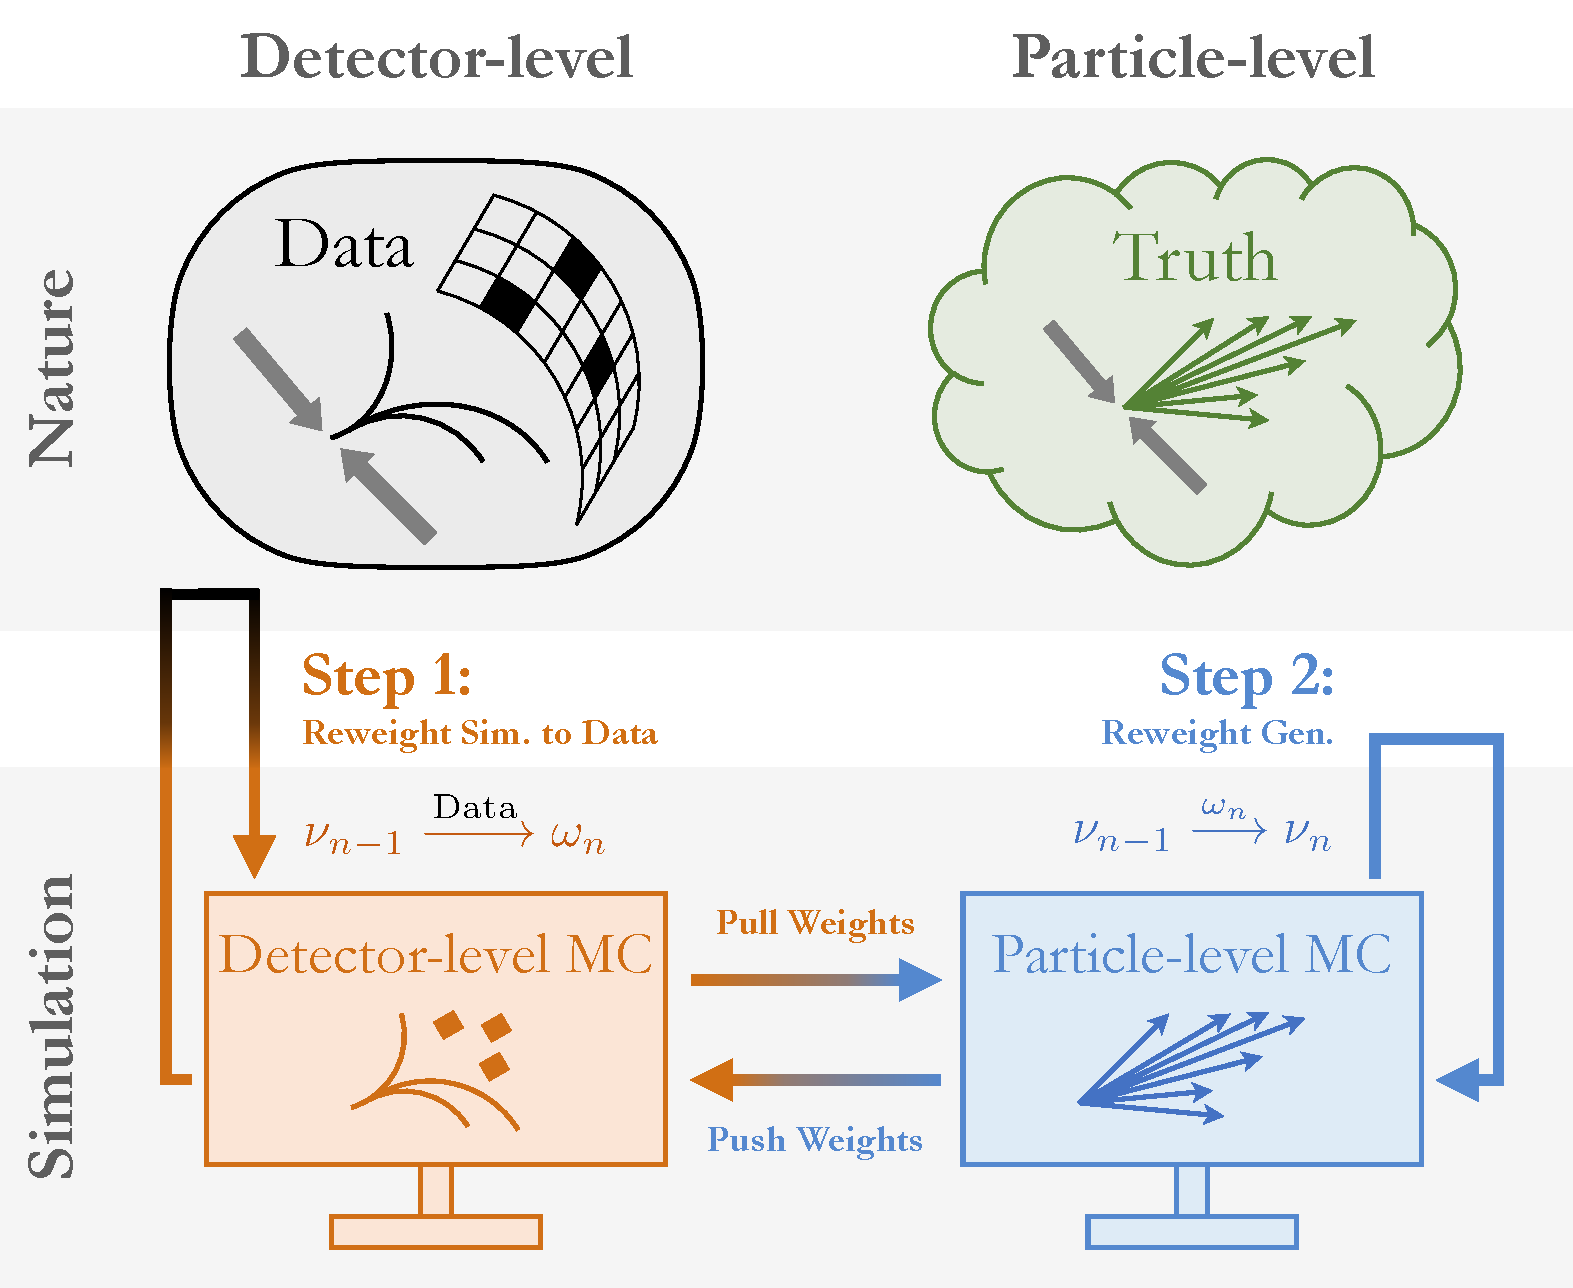
\includegraphics[width=0.6\textwidth]{Figures/schematic.pdf}
\caption{Figure adapted from Ref.~\cite{1911.09107}.}
\label{fig:omnifoldschematic}
\end{figure}

An effective strategy for implementing the OmniFold protocol is to use neural networks as reweighting functions.  A reweighting function is simply a ratio of two probability densities.  It is a fact that the optimal classifier between two event samples is the same quantity - the likelihood ratio (or any monotonic function of it).  Therefore, we build a reweighting function by training a classifier and properly interpreting the output.
In particular, a classifier $f$ trained using the standard binary cross entropy loss function on events with features $\vec{x}_i$ and event weights $w_i$
%
\begin{align}
\label{eq:binarycrossentropy}
        f^*=\argmin_f~~-\sum_{i\in\text{dataset 1}}w_i \log(f(\vec{x}_i)) -\sum_{i\in\text{dataset 2}} w_i\log(1-f(\vec{x}_i)),
\end{align}
%
has the property\footnote{This fact is well-known~\cite{hastie01statisticallearning,sugiyama_suzuki_kanamori_2012} and also has been used in many contexts in high-energy physics~\cite{2010.03569,1907.08209,Stoye:2018ovl,Hollingsworth:2020kjg,Brehmer:2018kdj,Brehmer:2018eca,Brehmer:2019xox,Brehmer:2018hga,Cranmer:2015bka,Badiali:2020wal,Andreassen:2020nkr,Andreassen:2019cjw,Fischer-ACAT2019}.} that asymptotically (i.e.\ with enough training data, flexible enough network architecture and training):
%
\begin{align}
\frac{f^*(\vec{x})}{1-f^*(\vec{x})}\propto \frac{p(\vec{x}|\text{dataset 1})}{p(\vec{x}|\text{dataset 2})}.
\end{align}
%
The proportionality is equality if the two datasets contain the same number of events; however, a constant is not important from the point of view of reweighting.

The power of neural networks is that they are naturally unbinned and can process high-dimensional data.  Furthermore, neural networks can also process variable-length data.  We will refer to the case that the inputs are one-dimensional as UniFold, the case that the inputs are multi- (but fixed-)dimensional as MultiFold, and the case where there are of variable dimension (namely, the raw particle data) as OmniFold.  If it is clear from context, we will simply refer to all of these approaches as OmniFold.

To develop an intuition for how OmniFold operates, the next section compares various approaches in a two-bin example where it is easy to derive the steps analytically.  Following that, we show a Gaussian example where the power of the neural network becomes clear.

\subsubsection{Illustration of Different Methods}

In order to illustrate the OmniFold procedure and how it compares to other techniques, it is useful to consider a simple two-bin example.  Suppose that there are only two possible values at particle-level and detector-level: $(T_1,T_2)$ and $(R_1,R_2)$, respectively.  The random variable $T_i$ is the number of events with a value $i$ at particle level (and similarly for $R_i$).  Further suppose that the detector response is given by:
%
\begin{align}
\Pr(R_1|T_1)&=100\%\,,\\
\Pr(R_1|T_2)&=50\%\,,
\end{align}
%
where $\Pr(x|y)$ is the conditional probability of $x$ given $y$.  The simulation has probability mass $\Pr_\text{MC}(T_i)=50\%$ so that $\Pr_\text{MC}(R_1)=75\%$ and $\Pr_\text{MC}(R_2)=25\%$.   Finally, we observe $\Pr_\text{Data}(R_1)=50\%$ in data.
With the notation used in Eq.~\ref{eq:foldingequation}, this situation is given by
%
\begin{eqnarray}
	\mathbf{R} = \begin{bmatrix} 1 & 0.5\\ 0 & 0.5\end{bmatrix}, & \mathbf{d} = \begin{bmatrix} 0.5\\ 0.5\end{bmatrix}, & \mathbf{c}=\mathbf{f}=\mathbf{1},~~\mathbf{b}=\mathbf{0}.
\end{eqnarray}
%
What do the various method predict for $\Pr_\text{unfolded}(T_1)$?   Before proceeding, note that the correct answer is $\Pr_\text{Data}(T_1)=0$, i.e.\ $\mathbf{t}=[0 1]^\intercal$.

\paragraph{OmniFold}  The first step of OmniFold is to derive weights $\omega_1$ to make the MC match the data.  The weight function is specified by two numbers, one for each of the two bin values.  These weights are given by $\omega_1(R_i)=\Pr_\text{Data}(R_i)/\Pr_\text{MC}(R_i)$, which is $\omega_1(R_1)=2/3$ and $\omega_1(R_2)=2$.  These weights are then pulled back to particle level.  In MC, 50\% of events have $(T_1,R_1)$, 25\% of events have $(T_2,R_1)$ and 25\% of events have $(T_2,R_2)$.   The first two of these types of events get assigned $\omega(R_1)$ and the last one gets assigned $\omega(R_2)$.  Therefore, the weighted particle-level probability mass function is $\Pr_\text{MC,1}(T_1)=1/3$.  The second step of OmniFold derives weights $\nu_1=\Pr_\text{MC,1}(T_i)/\Pr_\text{MC}(T_i)$, which are $\nu_1(T_1)=2/3$ and $\nu_1(T_2)=4/3$.

The above procedure is then repeated using the weights $\nu_1$ pushed to detector-level.  The new detector-level probability mass is given by $\Pr_\text{MC,2}(R_1)=2/3$.  Detector-level weights are derived according to $\omega_2(R_i)=\Pr_\text{Data}(R_i)/\Pr_\text{MC,2}(R_i)$.  Table~\ref{lab:omnifoldexample} shows the evolution of OmniFold over many iterations.

\begin{table}[h!]
\centering
\begin{tabular}{|ccccccc| }
\hline
$i$ & $\omega_i(R_1)$ & $\omega_i(R_2)$ & $\nu_i(R_1)$ & $\nu_i(R_2)$ & $\Pr_\text{MC,$i$}(R_1)$ & $\Pr_\text{MC,$i$}(T_1)$ \\
\hline
0 & 1 & 1 & 1 & 1 & $\sfrac{3}{4}$ & $\sfrac{1}{2}$ \\
1 & $\sfrac{2}{3}$ & $2$ & $\sfrac{2}{3}$ & $\sfrac{4}{3}$ & $\sfrac{2}{3}$ & $\sfrac{1}{3}$ \\
2 & $\sfrac{3}{4}$ & $\sfrac{3}{2}$ & $\sfrac{1}{2}$ & $\sfrac{3}{2}$ & $\sfrac{5}{8}$ & $\sfrac{1}{4}$ \\
\vdots & \vdots & \vdots & \vdots & \vdots & \vdots & \vdots \\
$\infty$ & 1 & 1 & 0 & 2 & \sfrac{1}{2} & 0\\
\hline
\end{tabular}
\caption{The evolution of OmniFold for the simple two-bin example described in the text.}
\label{lab:omnifoldexample}
\end{table}

\paragraph{Conditional GAN Unfolding (CGU)} In the training phase of CGU, one learns $\Pr(T_i|R_j)$ based on the simulation.  In the simple binned case, this probability mass is specified by four numbers.

\begin{align}
\Pr(T_i|R_j)&=\frac{\Pr(R_j|T_i)\Pr(T_i)}{\Pr(R_j|T_1)\Pr(T_1)+\Pr(R_j|T_2)\Pr(T_2)}\\
&=\frac{\Pr(R_j|T_i)}{\Pr(R_j|T_1)+\Pr(R_j|T_2)}\\
&=\left\{\begin{matrix}\sfrac{2}{3} & \text{$i=1$ and $j=1$} \cr 0 & \text{$i=1$ and $j=2$}  \cr \sfrac{1}{3}& \text{$i=2$ and $j=1$}  \cr 1& \text{$i=2$ and $j=2$}  \end{matrix}\right.
\end{align}
%
Applied to data, we would measure
%
\begin{align}
\Pr{}_\text{unfolded}(T_1)&=\Pr(T_1|R_1)\Pr{}_\text{data}(R_1)+\Pr(T_1|R_2)\Pr{}_\text{data}(R_2)=\sfrac{1}{6}\,,\\
\Pr{}_\text{unfolded}(T_2)&=\Pr(T_2|R_1)\Pr{}_\text{data}(R_1)+\Pr(T_2|R_2)\Pr{}_\text{data}(R_2)=\sfrac{5}{6}\,,
\end{align}
%
which is the wrong answer.

\paragraph{Conditional Normalizing Flow Unfolding (CNFU)} In the binned case, this is equivalent to matrix inversion.   The response matrix is

\begin{align}
\mathbf{R}=\begin{pmatrix} 1& \sfrac{1}{2}\cr 0 & \sfrac{1}{2}\end{pmatrix}\implies \mathbf{R}^{-1}=\begin{pmatrix} 1 & -1 \cr 0 & 2\end{pmatrix}\,.
\end{align}
%
Applying $\mathbf{R}^{-1}$ to $(\sfrac{1}{2},\sfrac{1}{2}$) results in $(0,1)$, the correct answer.  There are many undesirable features of matrix inversion, but it does result in an unbiased measurement.

\paragraph{Iterative Bayesian Unfolding (IBU)}

Table~\ref{lab:ibuexample} shows the evolution of IBU over many iterations.  Note that the second column of Table~\ref{lab:ibuexample} is the same as the last column of Table~\ref{lab:omnifoldexample} - this is because OmniFold and IBU are equivalent in the binned case.

\begin{table}[h!]
\centering
\begin{tabular}{|cccccc| }
\hline
$i$ & $\Pr_\text{MC,$i$}(T_1)$ & $\Pr_0(T_1|M_1)$ & $\Pr_0(T_1|M_2)$ & $\Pr_0(T_2|M_1)$ & $\Pr_0(T_2|M_2)$\\
\hline
$0$ & $\sfrac{1}{2}$ & $\sfrac{2}{3}$ & 0 & $\sfrac{1}{3}$ & $1$\\
$1$ & $\sfrac{1}{3}$ & $\sfrac{1}{2}$ & 0 & $\sfrac{1}{2}$ & $1$\\
$2$ & $\sfrac{1}{4}$ & $\sfrac{2}{5}$ & 0 & $\sfrac{3}{5}$ & $1$\\
\vdots & \vdots & \vdots & \vdots & \vdots & \vdots  \\
$\infty$ & 0 & 0 & 0 & 1 & 1\\
\hline
\end{tabular}
\caption{The evolution of IBU for the simple two-bin example described in the text.}
\label{lab:ibuexample}
\end{table}

\subsection{Gaussian Example}
\label{sec:gaus}

This section shows the unfolding of a one-dimensional Gaussian random variable with a Gaussian noise model.  Figure~\ref{fig:gaussian:inputs} shows the `data' and `simulation'.  The data has a mean of 1 and a standard deviation of 1.5 while the simulation has a mean of 0 and a standard deviation of 1.  In both cases, the distributions are made up of ten million events and the detector effects (noise) are an additive Gaussian with mean 0 and unit variance.

The neural network implemented for reweighting is comprised of 3 layers, with 50 nodes per layer.  Rectified linear units (ReLU) connect the intermediate layers and the output is Softmax.  The training/validation split is 75/25.  The network is trained for 200 epochs with early stopping using a patience of 10\footnote{The training ends if the validation loss is not improved for 10 epochs.  The network weights with the lowest validation loss are restored.}, and the training time is about 5 seconds per epoch on an NVIDIA Quadro RTX 6000 GPU. The batch size is $10^5$.  All neural networks are implemented using \textsc{Keras}~\cite{keras} with the \textsc{Tensorflow} backend~\cite{tensorflow} and optimized with \textsc{Adam}~\cite{adam}.  Networks are trained using the binary cross entropy loss function described in Eq.~\ref{eq:binarycrossentropy}.

Six iterations resulting in successful unfolding using the OmniFold procedure is demonstrated in Fig.~\ref{fig:gaussian:iterations}.

To model the effects of initial Monte Carlo (MC) generation event weights, we inject artificial initial event weights. Specifically, each event in the particle-level truth and particle-level simulation $x_i$ is given a weight $w_i$ with $w_i$ drawn from $\mathcal{N}(x_i, 1)$; effectively, events further from the origin are more heavily weighted. This results in the distributions shown in Figure~\ref{fig:gaussian:MCinputs}. We then carry out an identical unfolding procedure as described above, simply initializing $\omega_0$ as the initial event weights $w_i$ for simulation.

Again, six iterations resulting in successful unfolding using the OmniFold procedure for the case with initial MC weights injected is demonstrated in Fig.~\ref{fig:gaussian:MCiterations}.

\begin{figure}[h!]
\centering
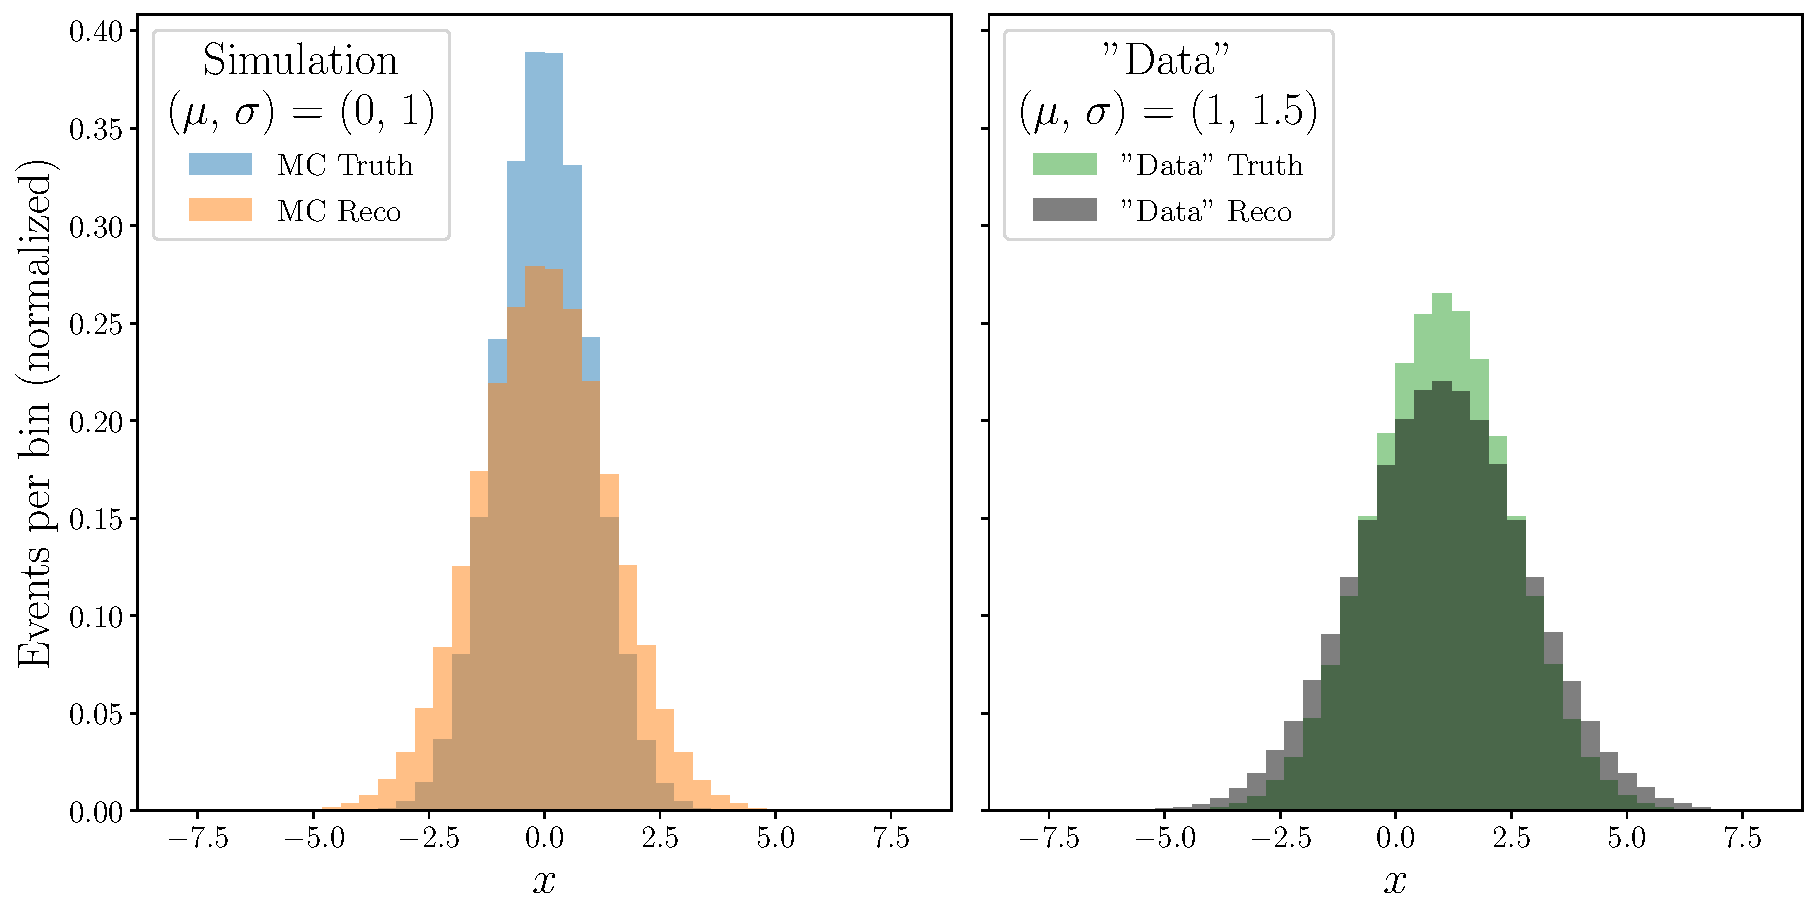
\includegraphics[width=0.6\textwidth]{Figures/GaussianToyExample/GaussianToyExample-Distributions.pdf}
\caption{The `simulation' (left) and `data' (right) for the one-dimensional Gaussian illustration.  The narrower histograms are the particle-level distributions and the wider ones are the detector-level distributions.}
\label{fig:gaussian:inputs}
\end{figure}

\begin{figure}[h!]
\centering
\subfloat[1 iteration]{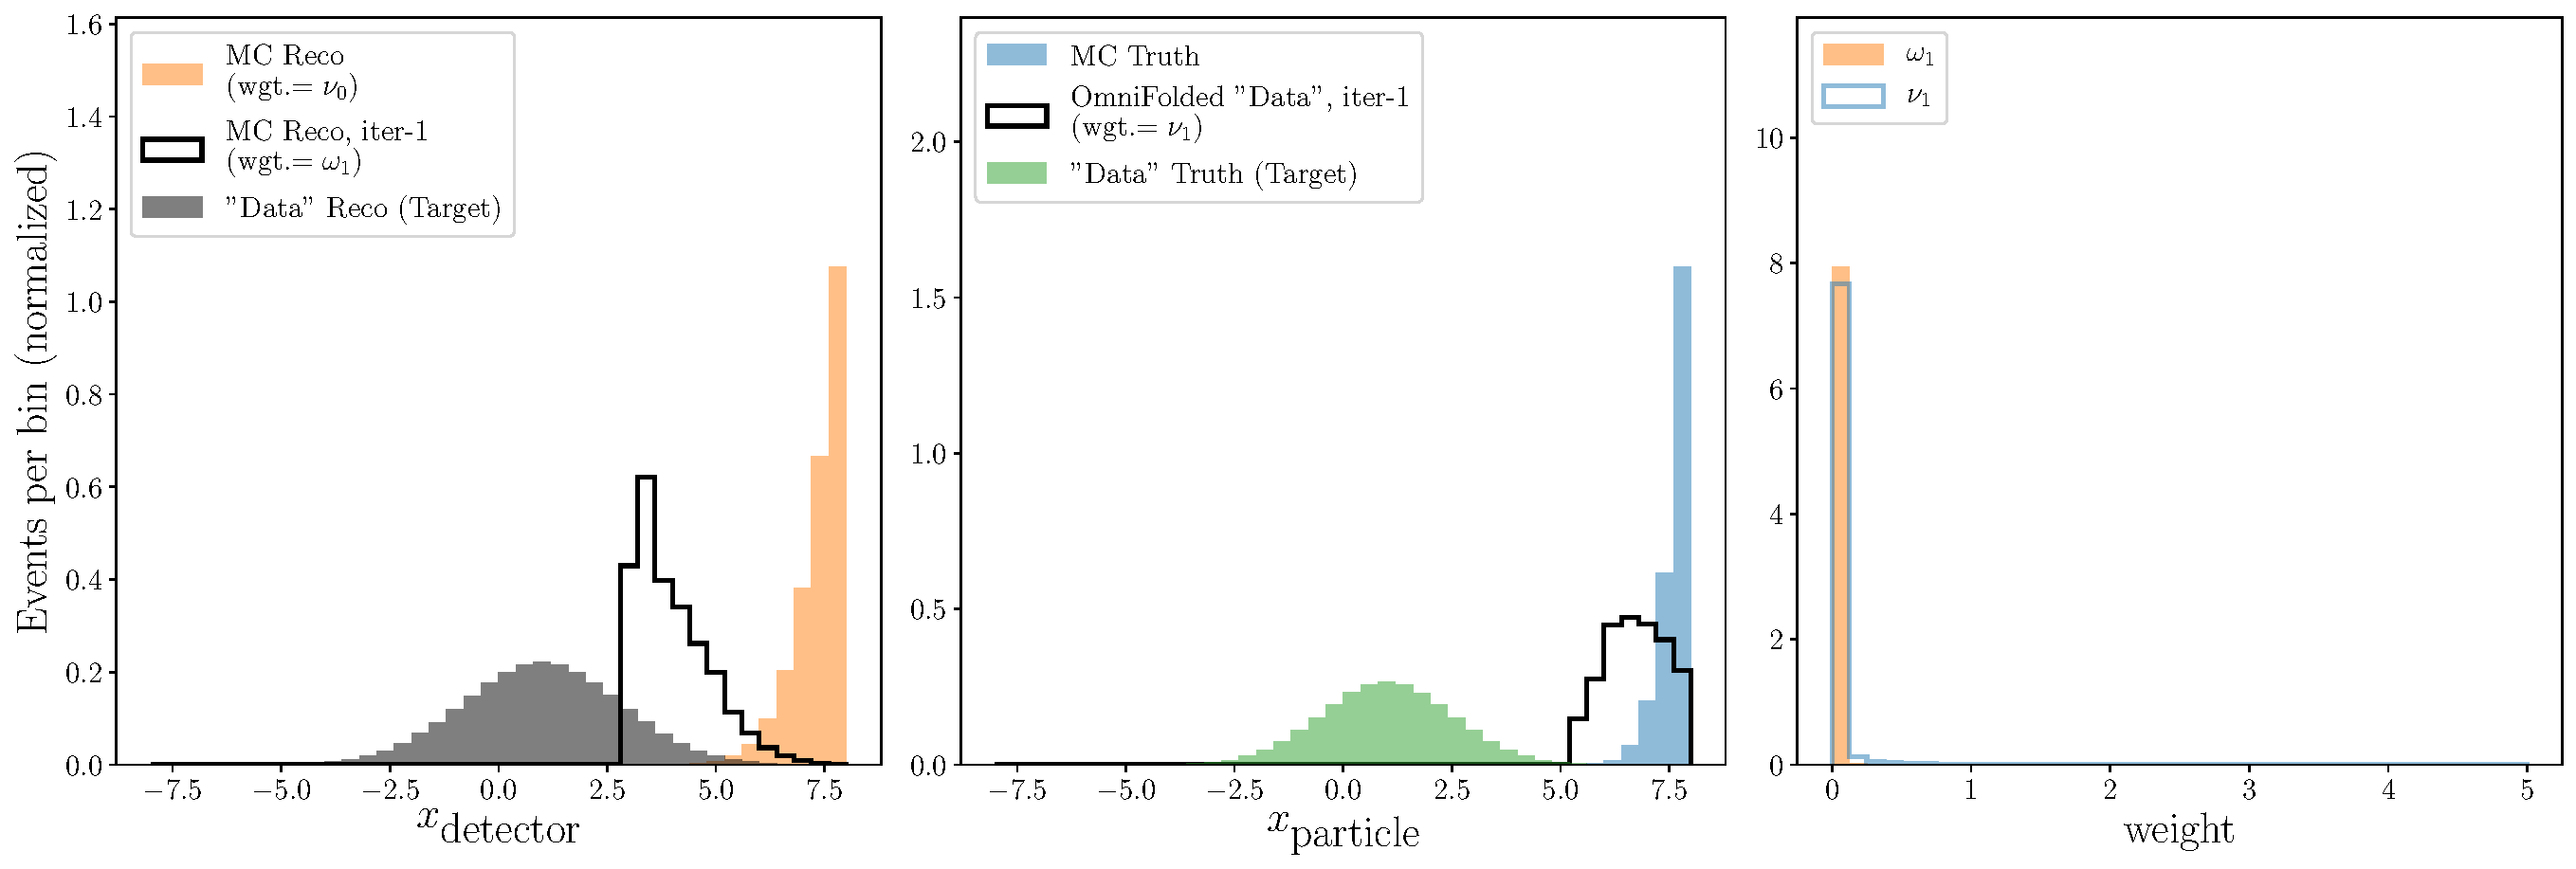
\includegraphics[width=0.45\textwidth]{Figures/GaussianToyExample/GaussianToyExample-UnfoldingResultsIteration01.pdf}}\subfloat[2 iterations]{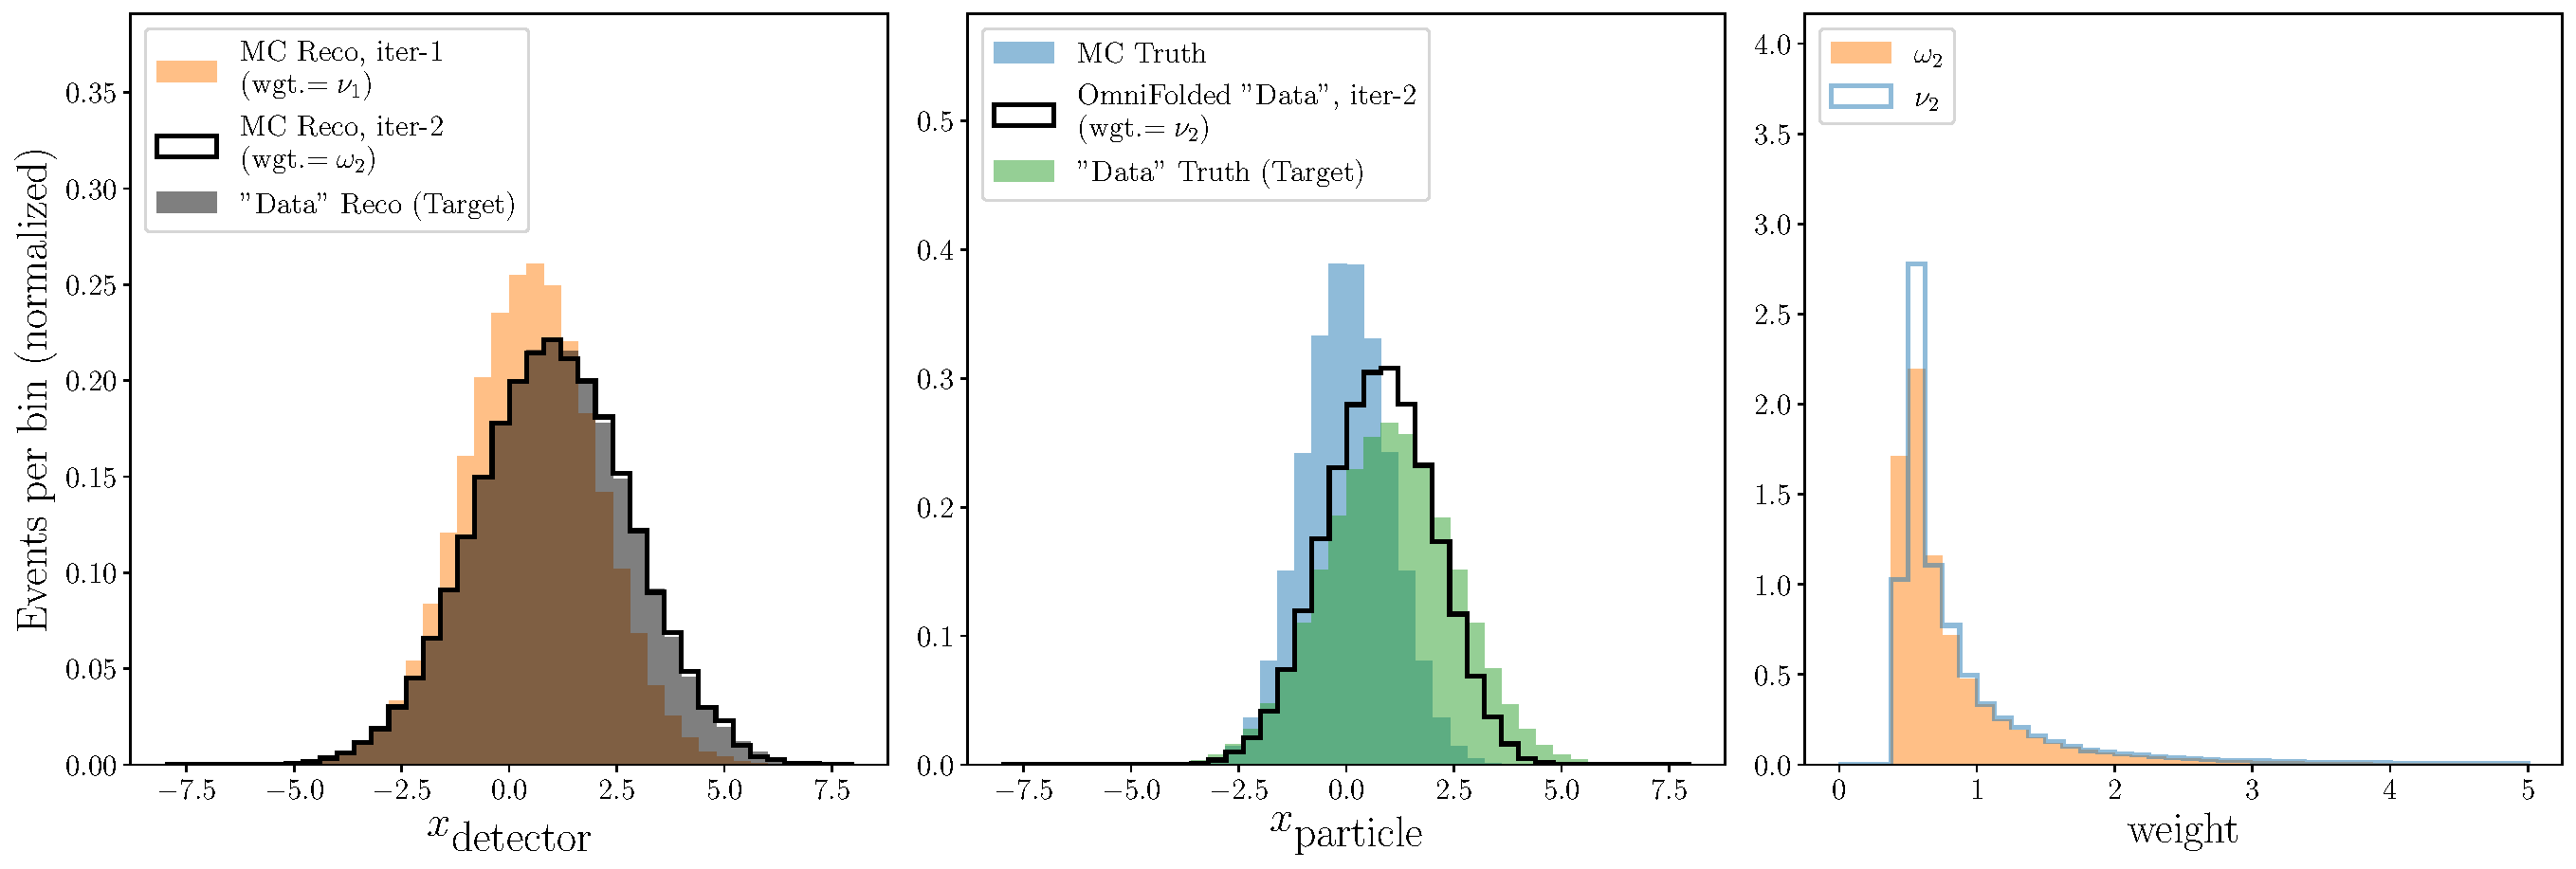
\includegraphics[width=0.45\textwidth]{Figures/GaussianToyExample/GaussianToyExample-UnfoldingResultsIteration02.pdf}}\\
\subfloat[3 iterations]{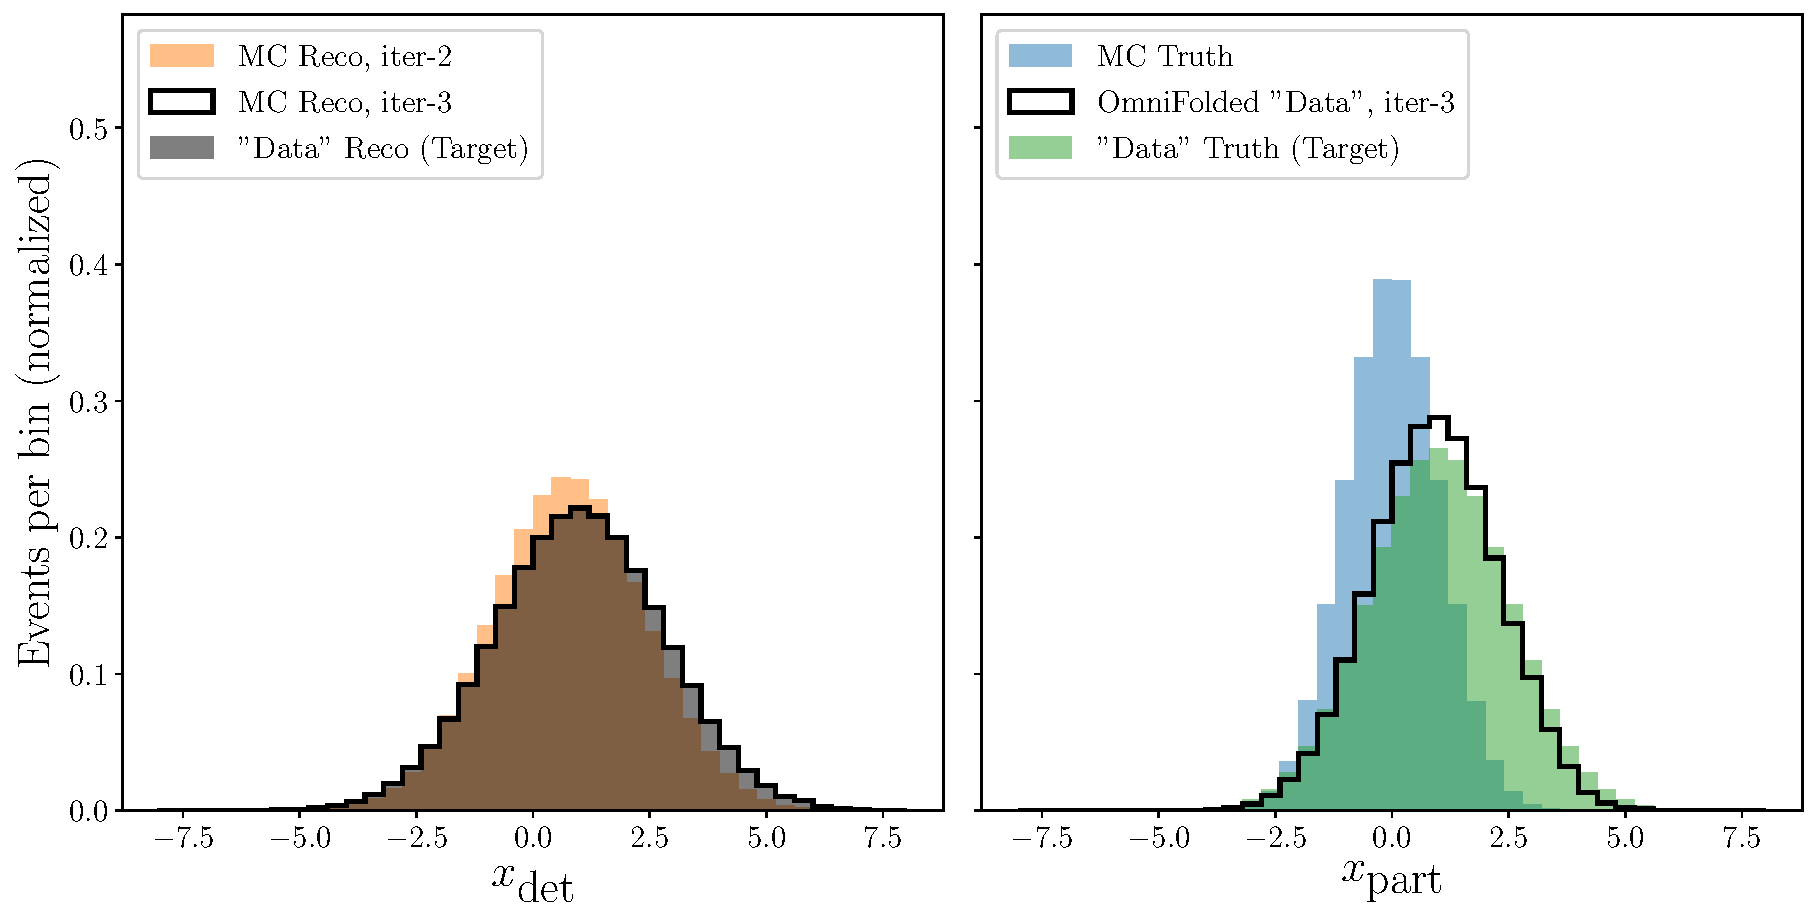
\includegraphics[width=0.45\textwidth]{Figures/GaussianToyExample/GaussianToyExample-UnfoldingResultsIteration03.pdf}}\subfloat[4 iterations]{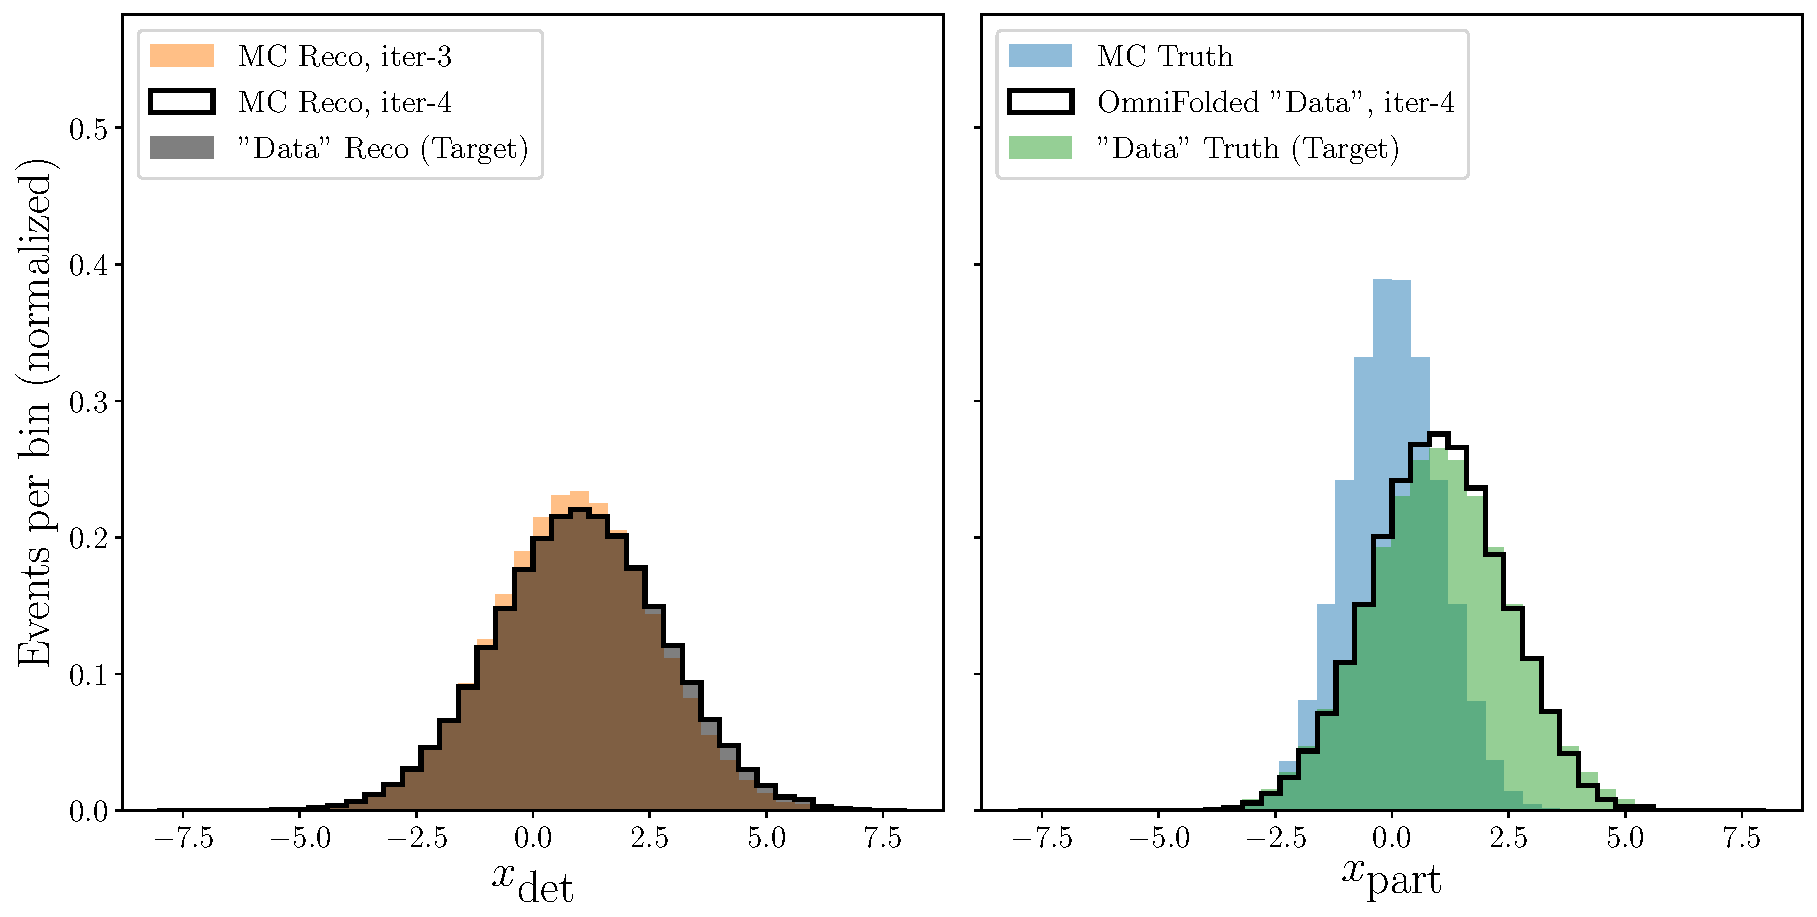
\includegraphics[width=0.45\textwidth]{Figures/GaussianToyExample/GaussianToyExample-UnfoldingResultsIteration04.pdf}}\\
\subfloat[5 iterations]{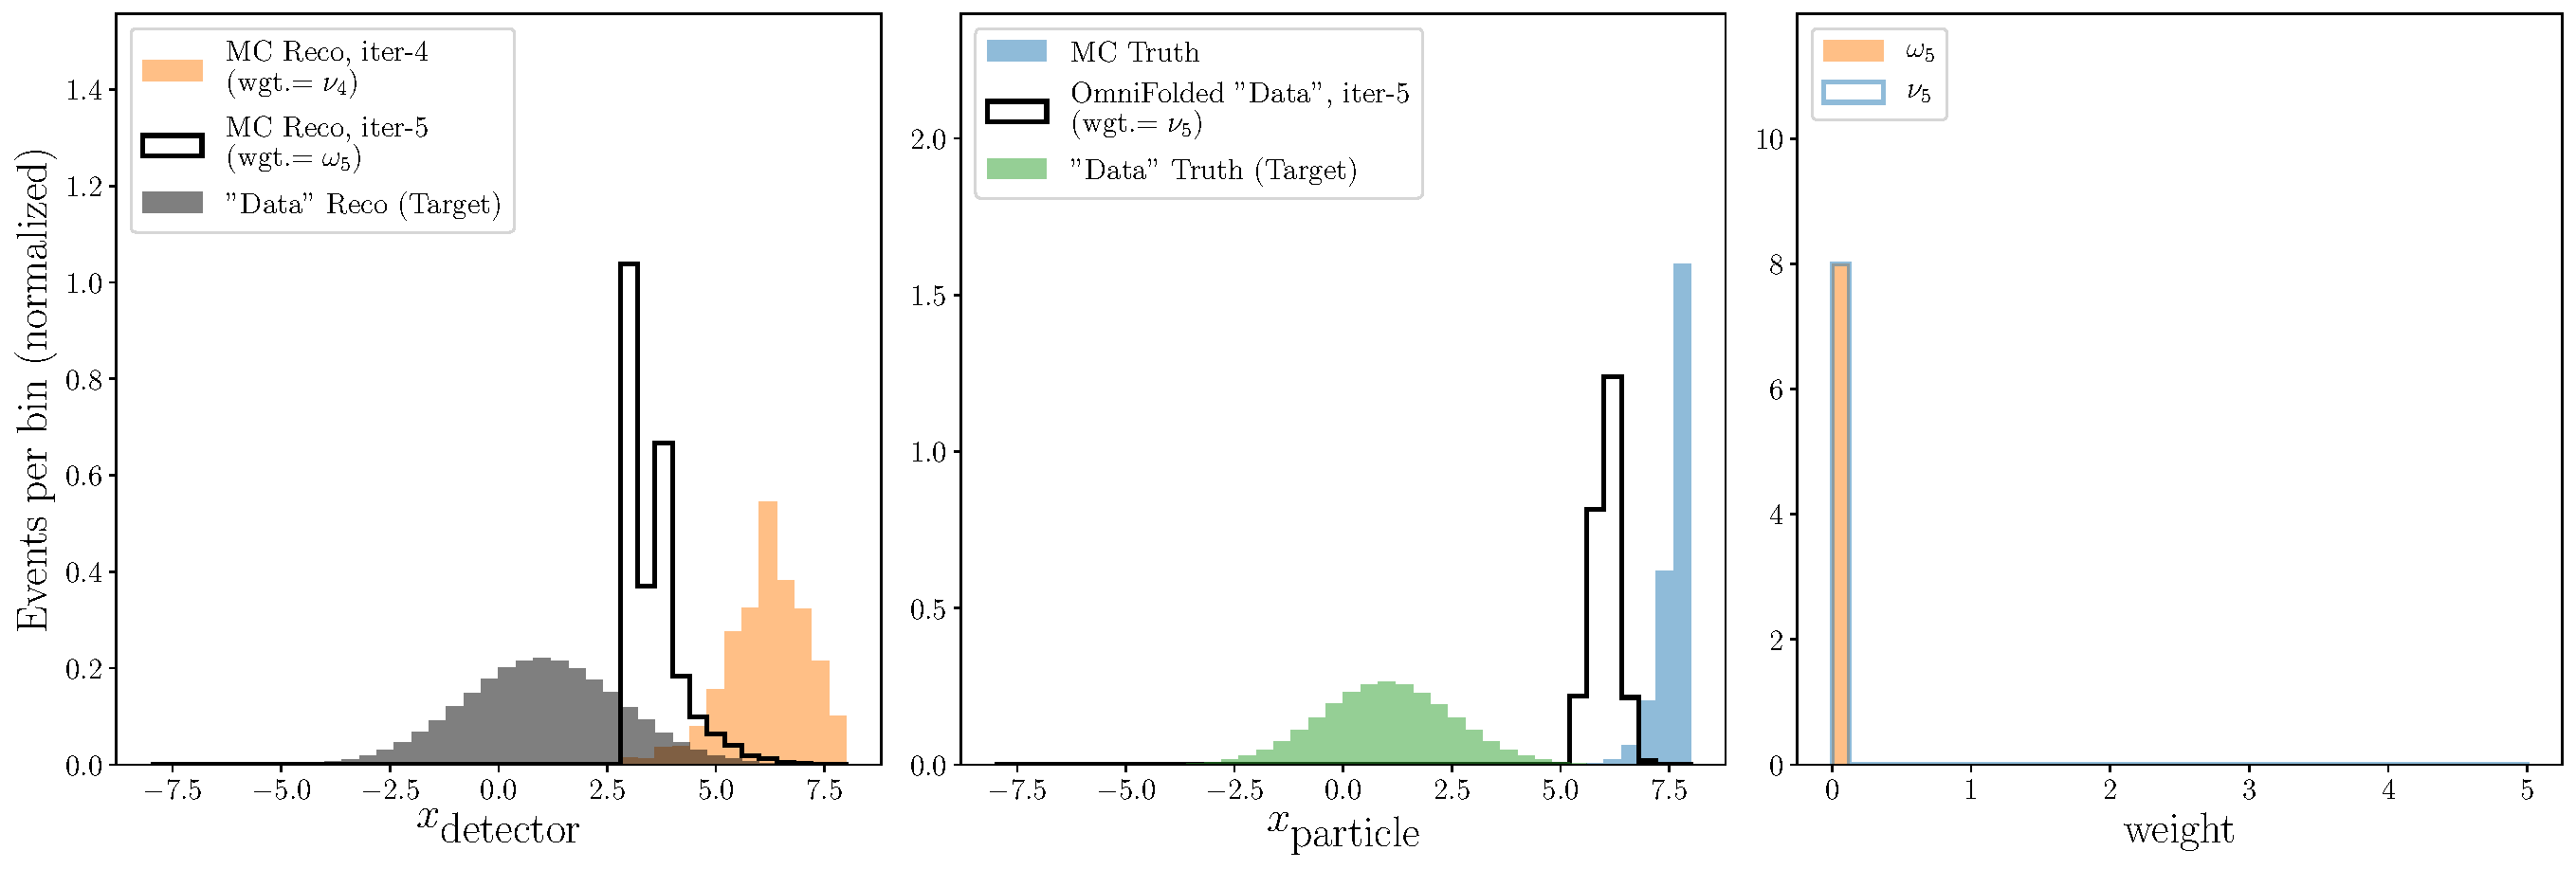
\includegraphics[width=0.45\textwidth]{Figures/GaussianToyExample/GaussianToyExample-UnfoldingResultsIteration05.pdf}}\subfloat[6 iterations]{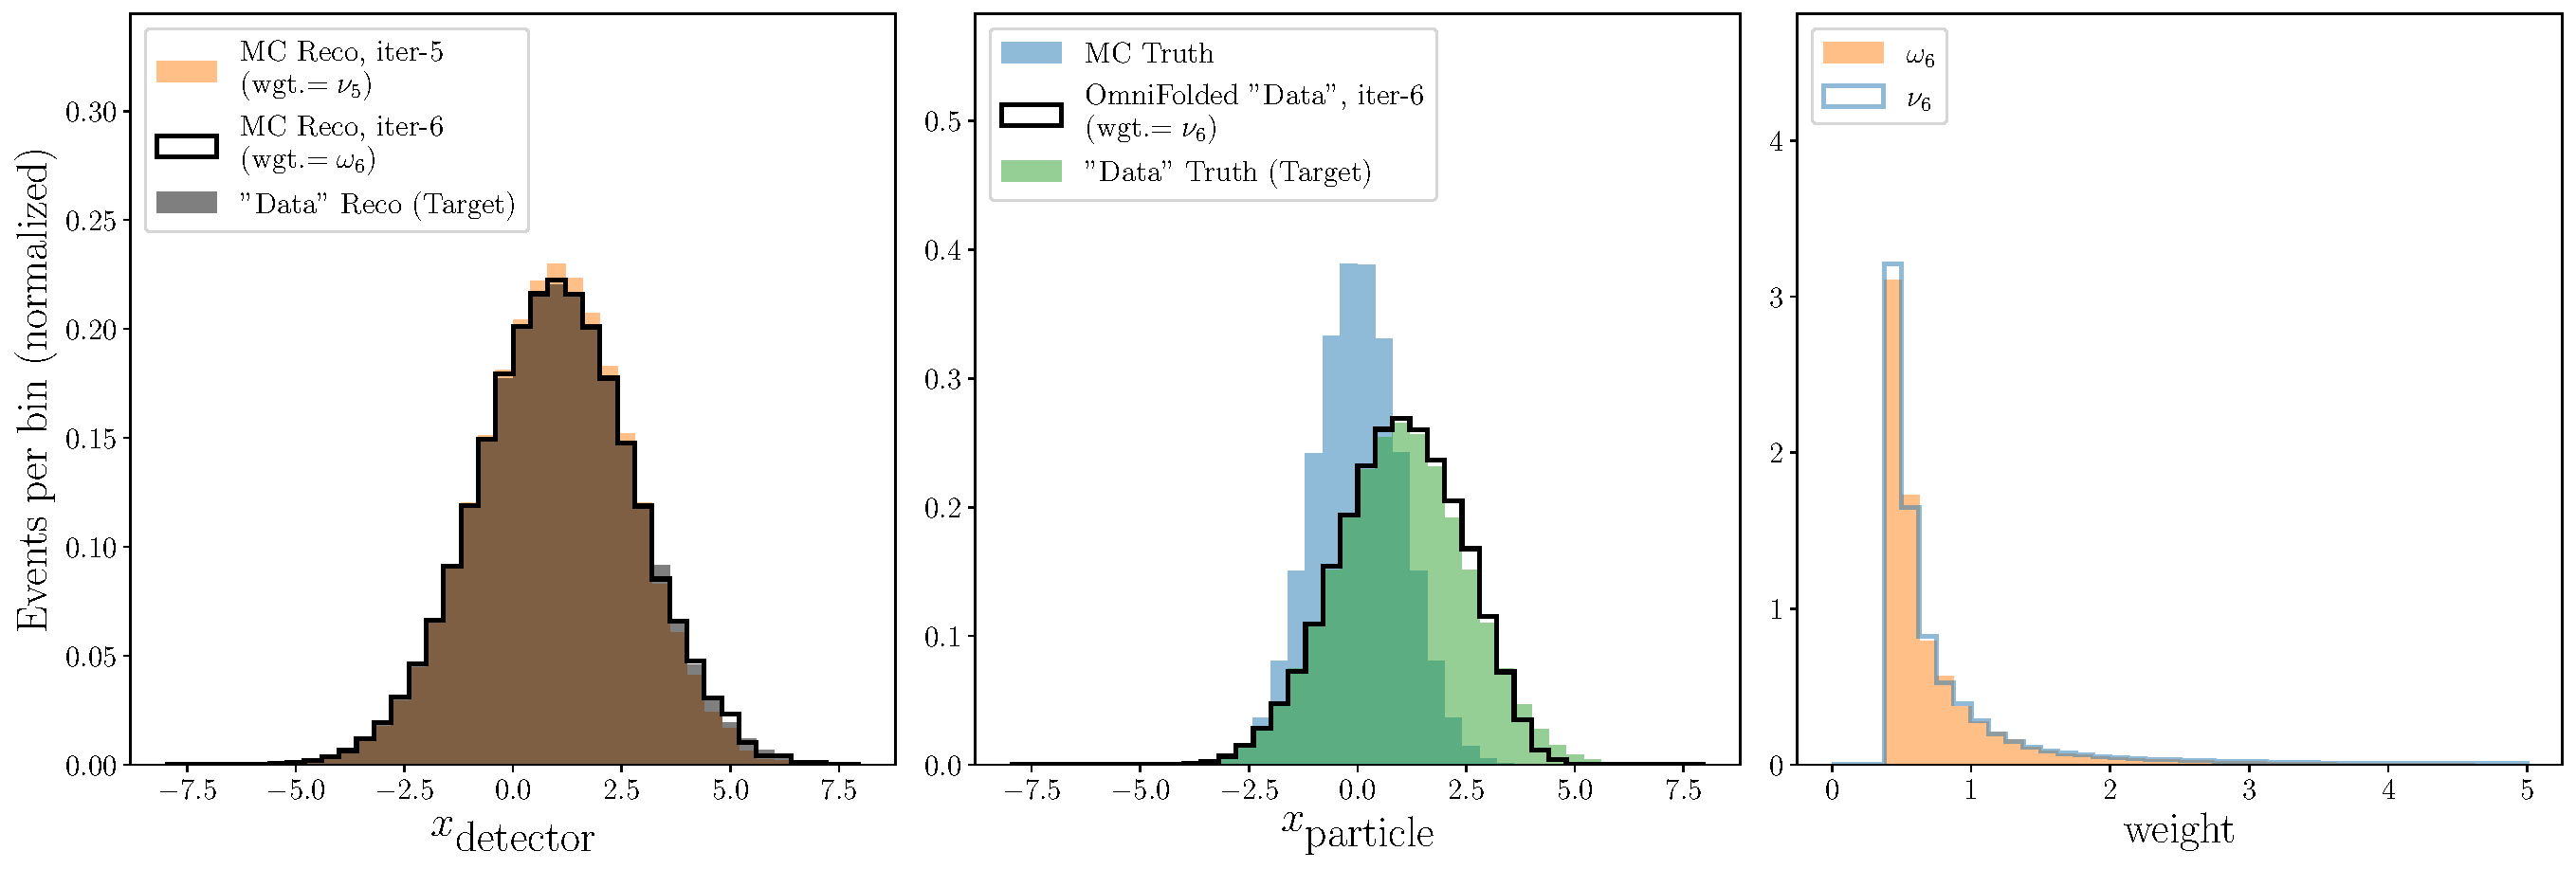
\includegraphics[width=0.45\textwidth]{Figures/GaussianToyExample/GaussianToyExample-UnfoldingResultsIteration06.pdf}}
\caption{An illustration of six iterations of the OmniFold algorithm to the one-dimensional Gaussian example.  For each iteration, the left plot is the detector-level distribution with weights $\omega_n$ and the right plot is the particle-level distribution with weights $\nu_n$.}
\label{fig:gaussian:iterations}
\end{figure}

\begin{figure}[h!]
\centering
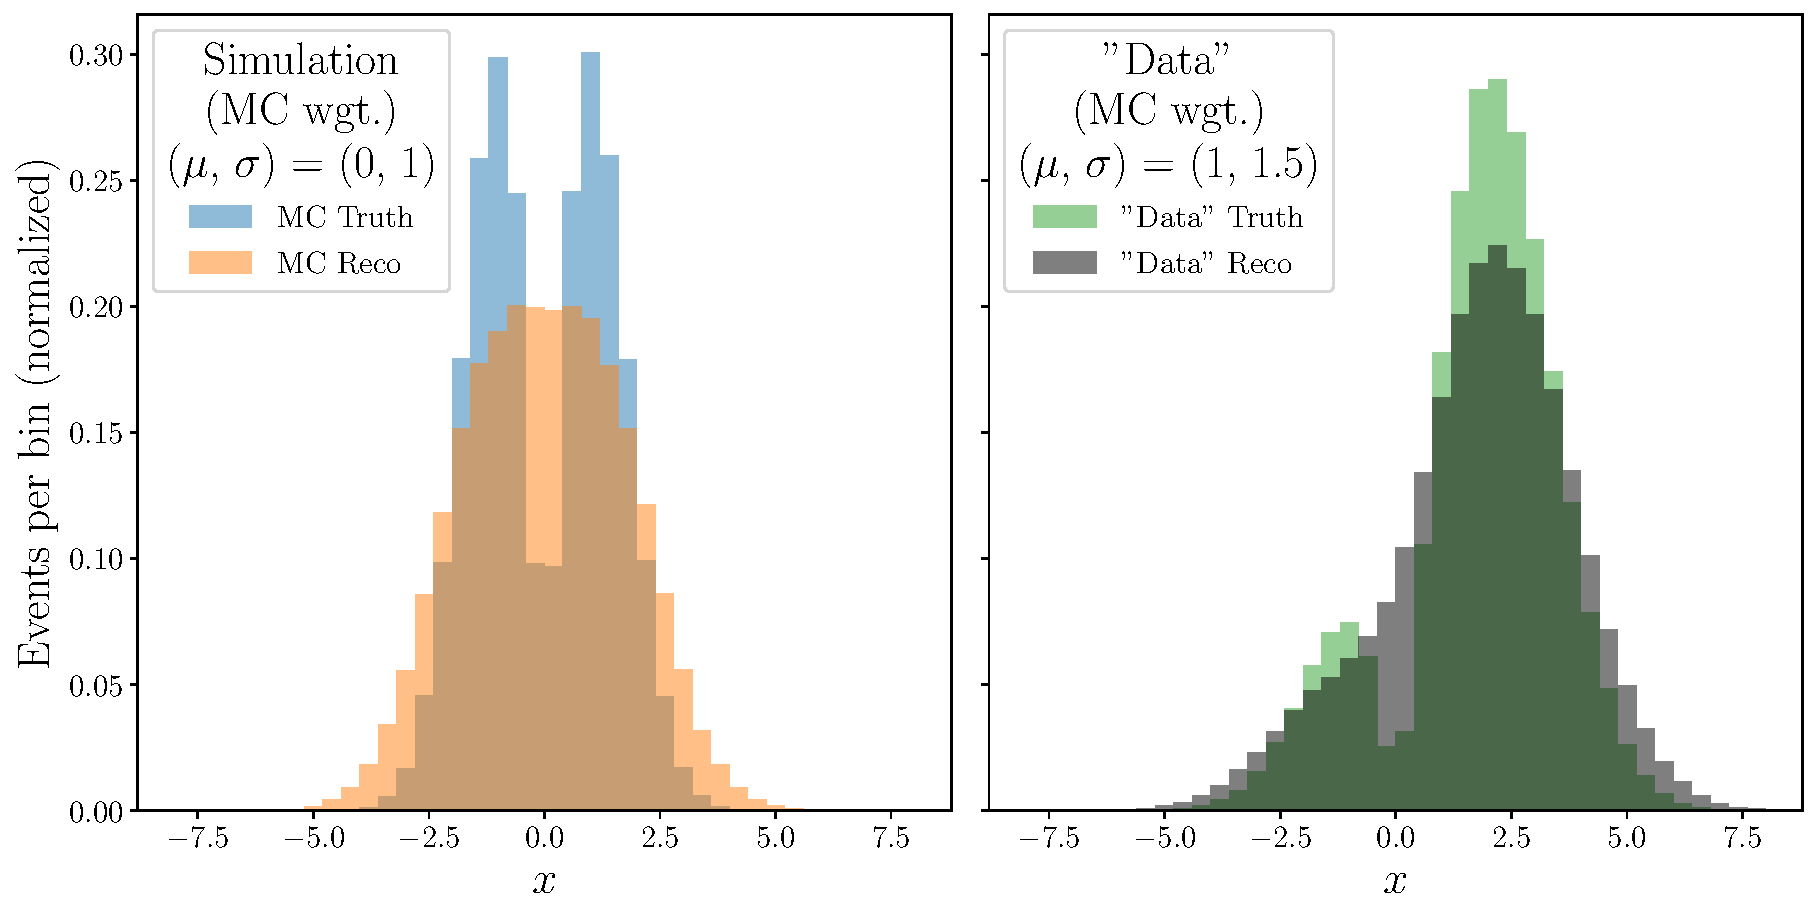
\includegraphics[width=0.6\textwidth]{Figures/GaussianToyExample/GaussianToyExample-MCDistributions.pdf}
\caption{The `simulation' (left) and `data' (right) for the one-dimensional Gaussian illustration with initial MC event weights included.}
\label{fig:gaussian:MCinputs}
\end{figure}

\begin{figure}[h!]
\centering
\subfloat[1 iteration]{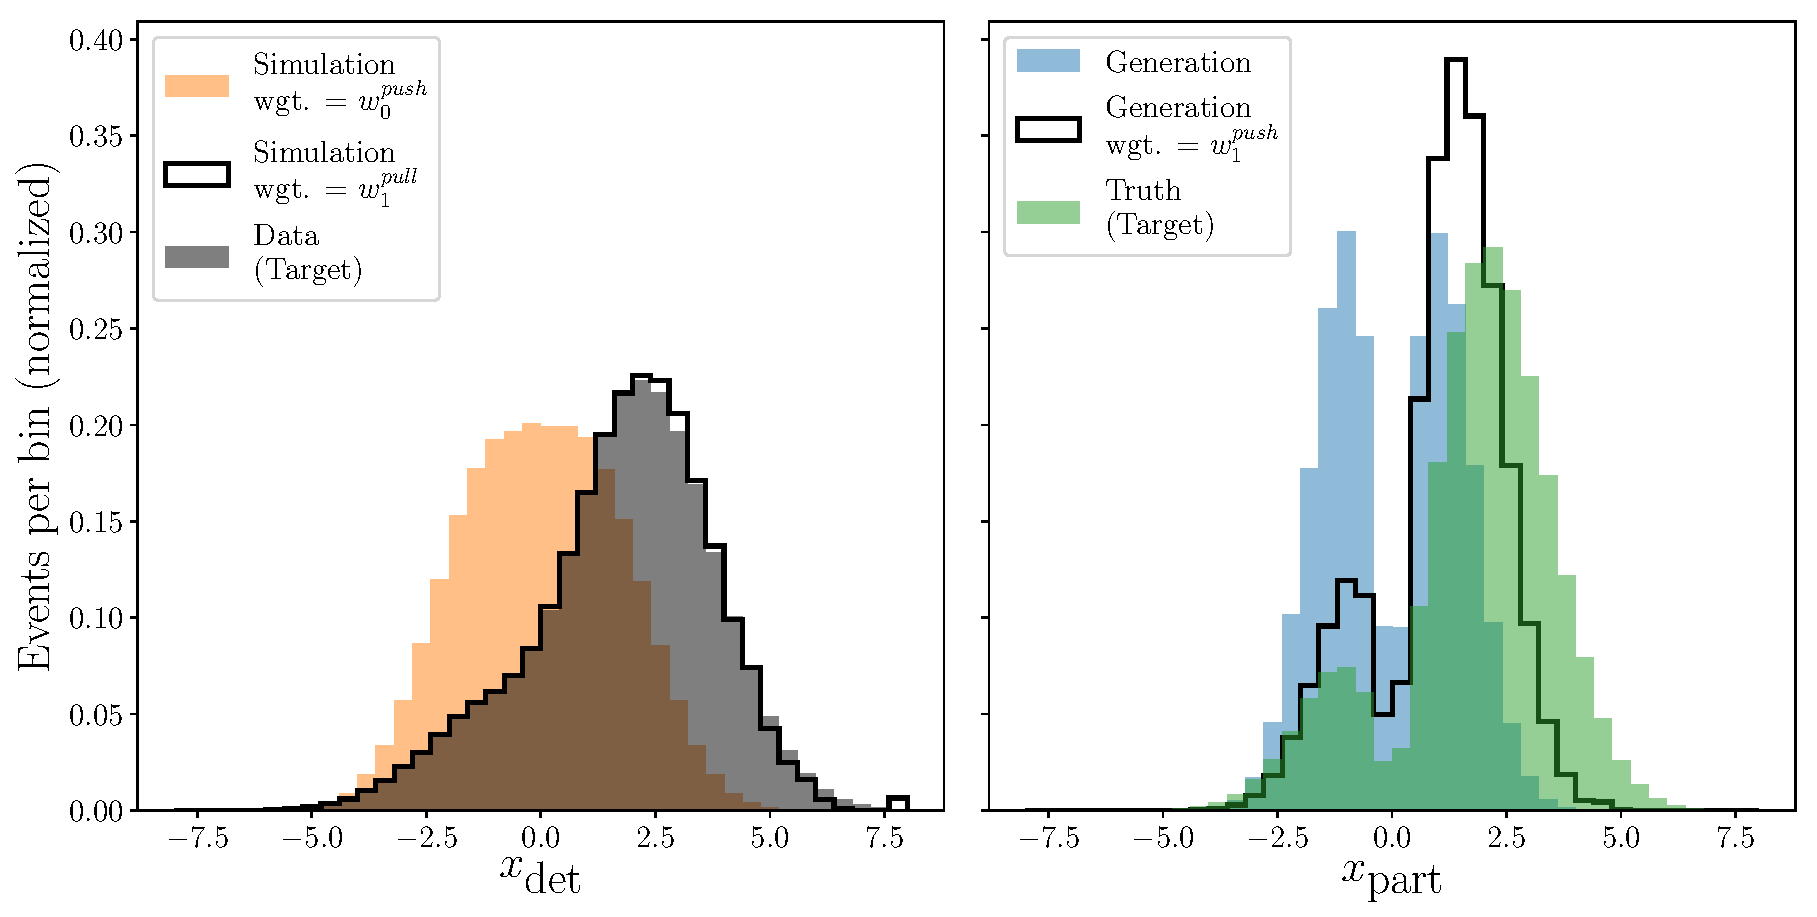
\includegraphics[width=0.45\textwidth]{Figures/GaussianToyExample/GaussianToyExample-MCUnfoldingResultsIteration01.pdf}}\subfloat[2 iterations]{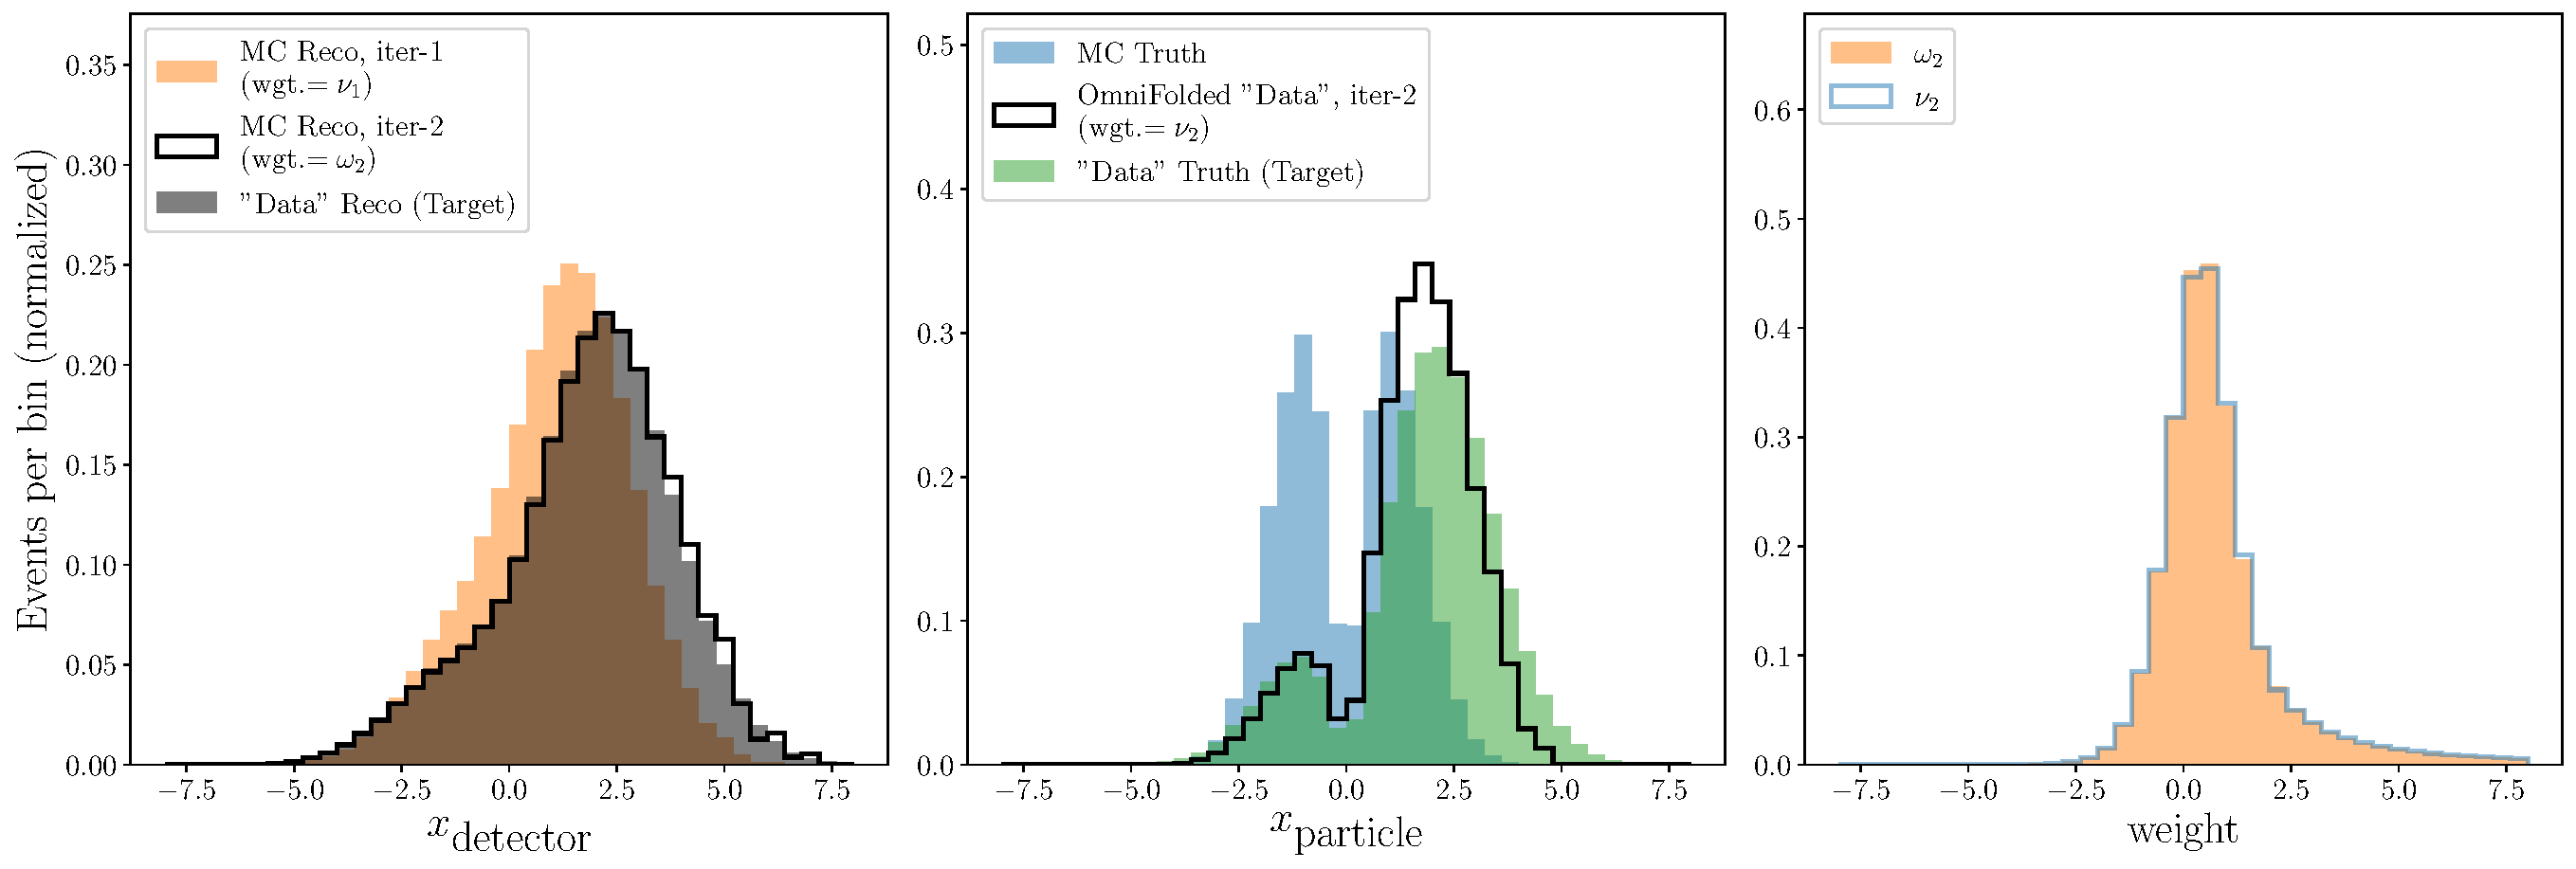
\includegraphics[width=0.45\textwidth]{Figures/GaussianToyExample/GaussianToyExample-MCUnfoldingResultsIteration02.pdf}}\\
\subfloat[3 iterations]{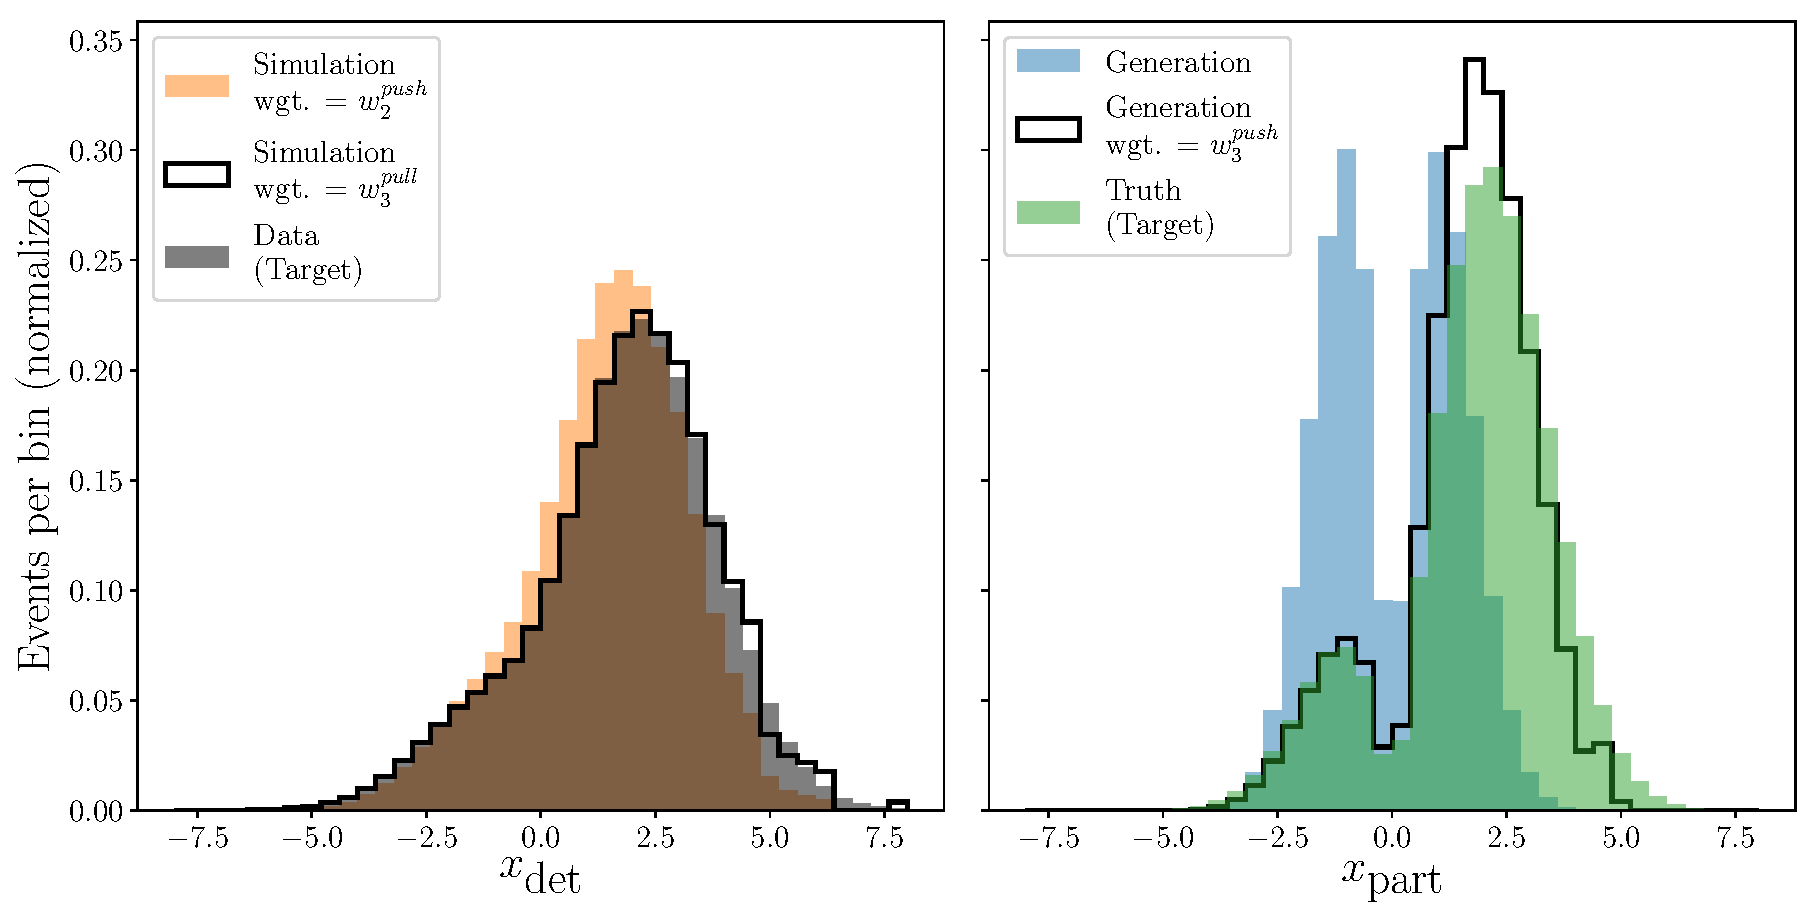
\includegraphics[width=0.45\textwidth]{Figures/GaussianToyExample/GaussianToyExample-MCUnfoldingResultsIteration03.pdf}}\subfloat[4 iterations]{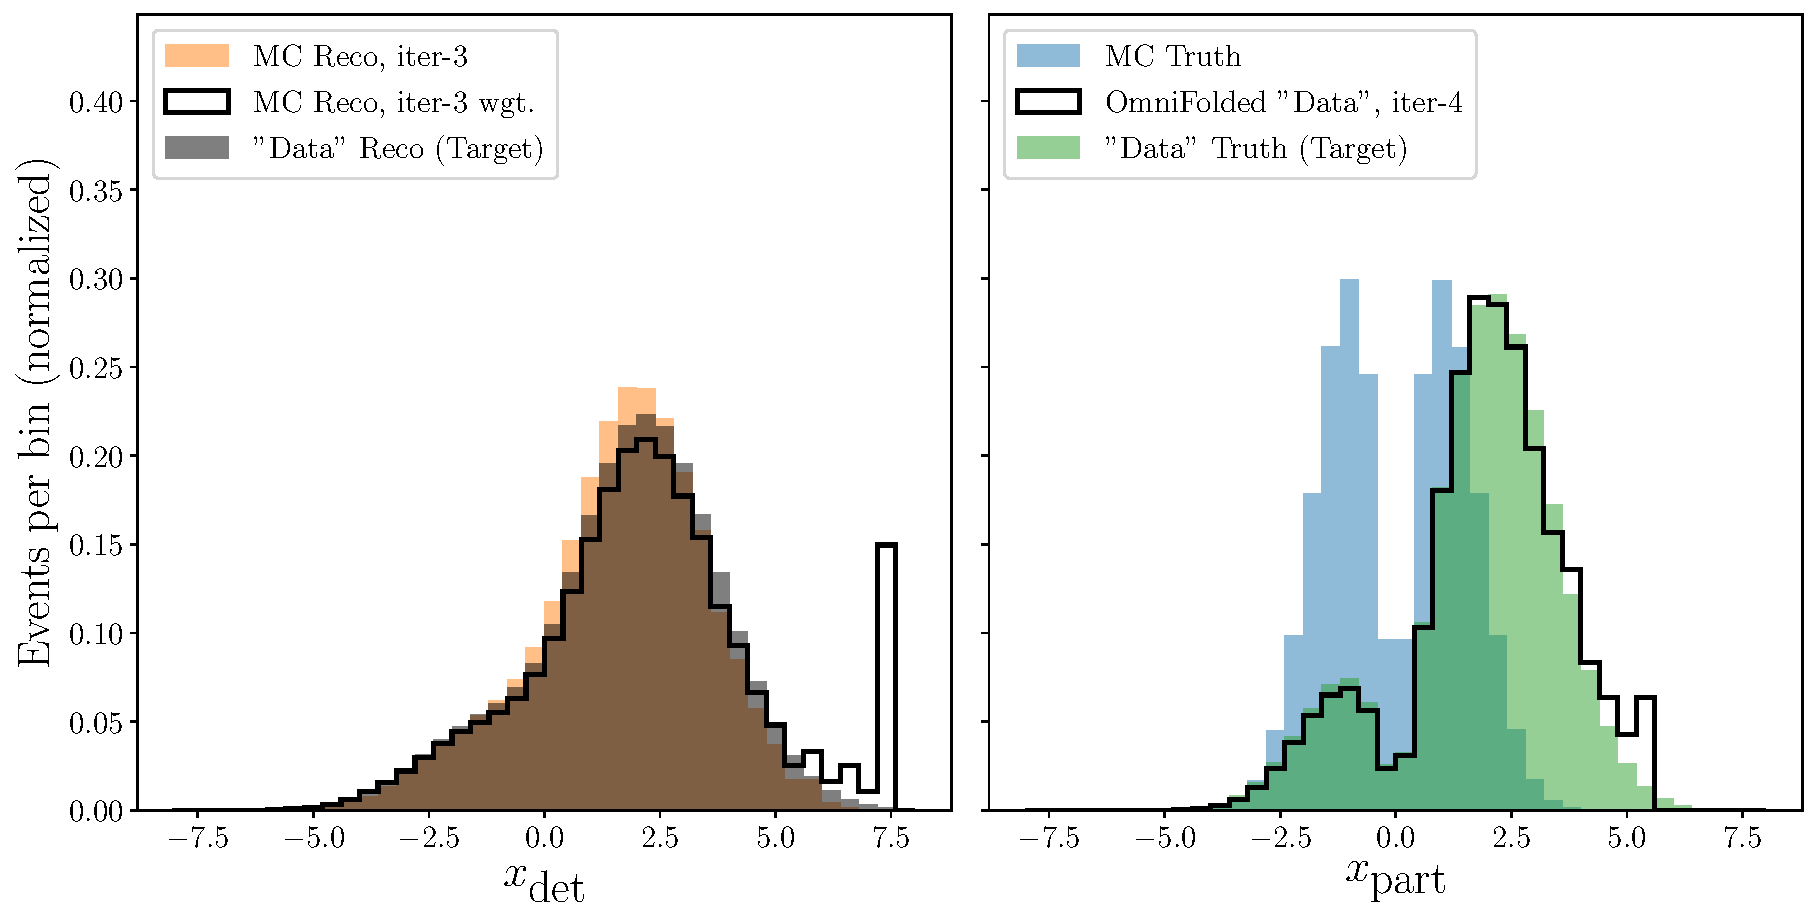
\includegraphics[width=0.45\textwidth]{Figures/GaussianToyExample/GaussianToyExample-MCUnfoldingResultsIteration04.pdf}}\\
\subfloat[5 iterations]{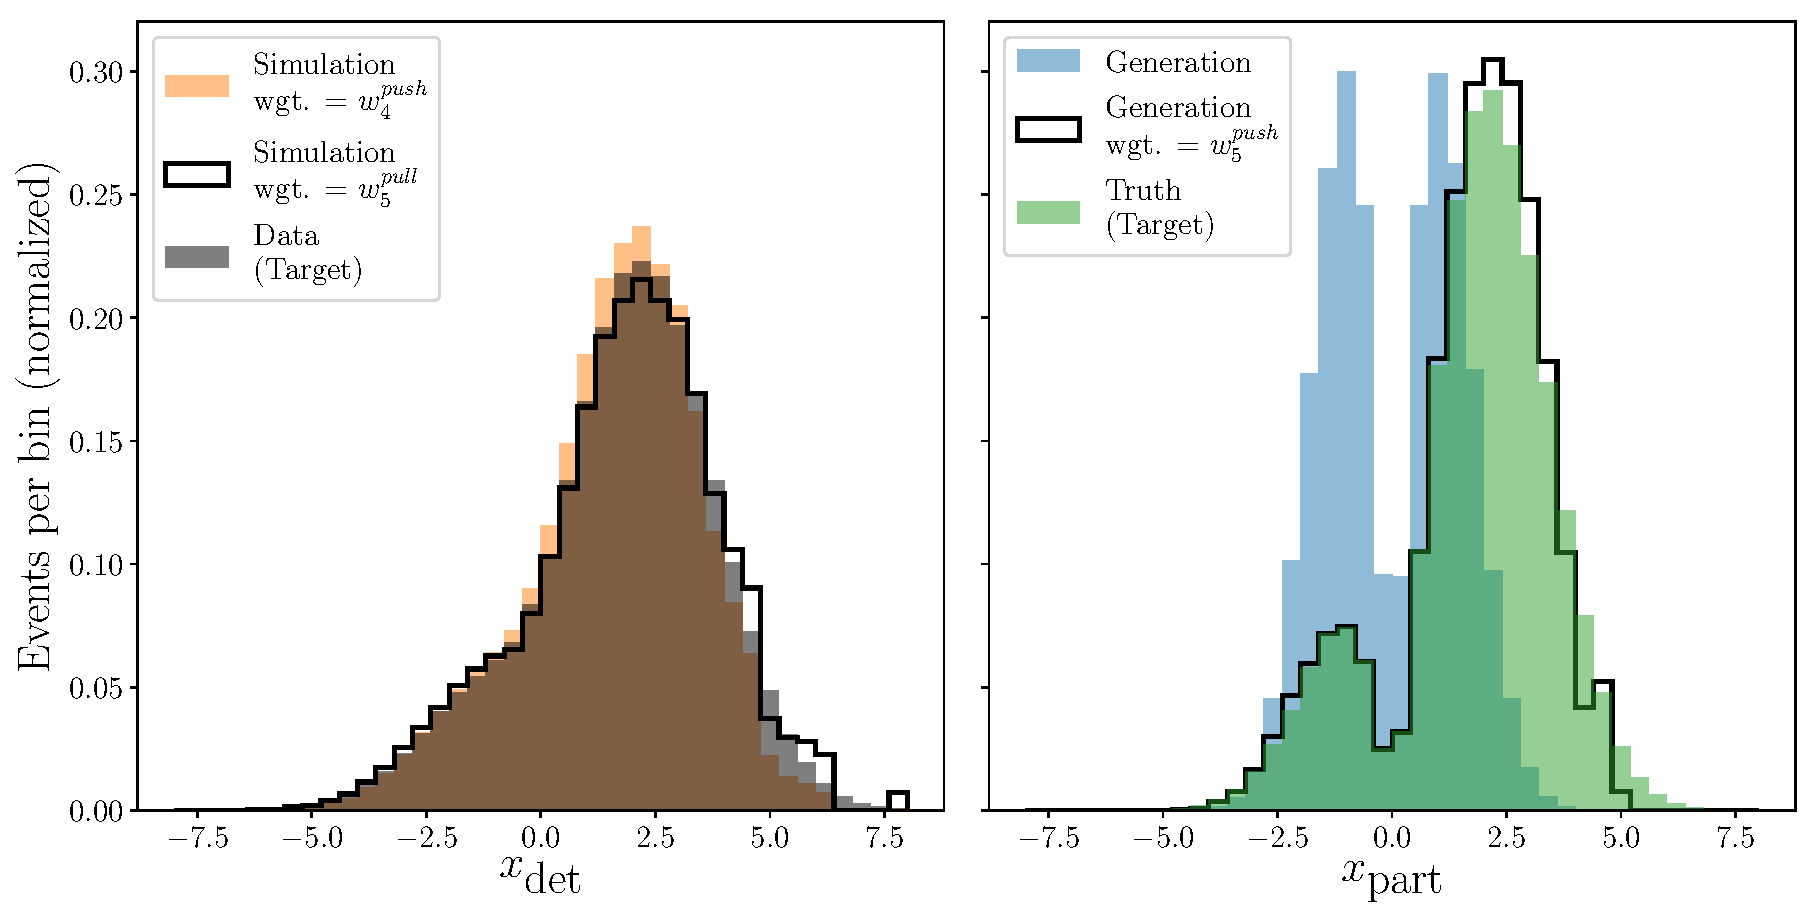
\includegraphics[width=0.45\textwidth]{Figures/GaussianToyExample/GaussianToyExample-MCUnfoldingResultsIteration05.pdf}}\subfloat[6 iterations]{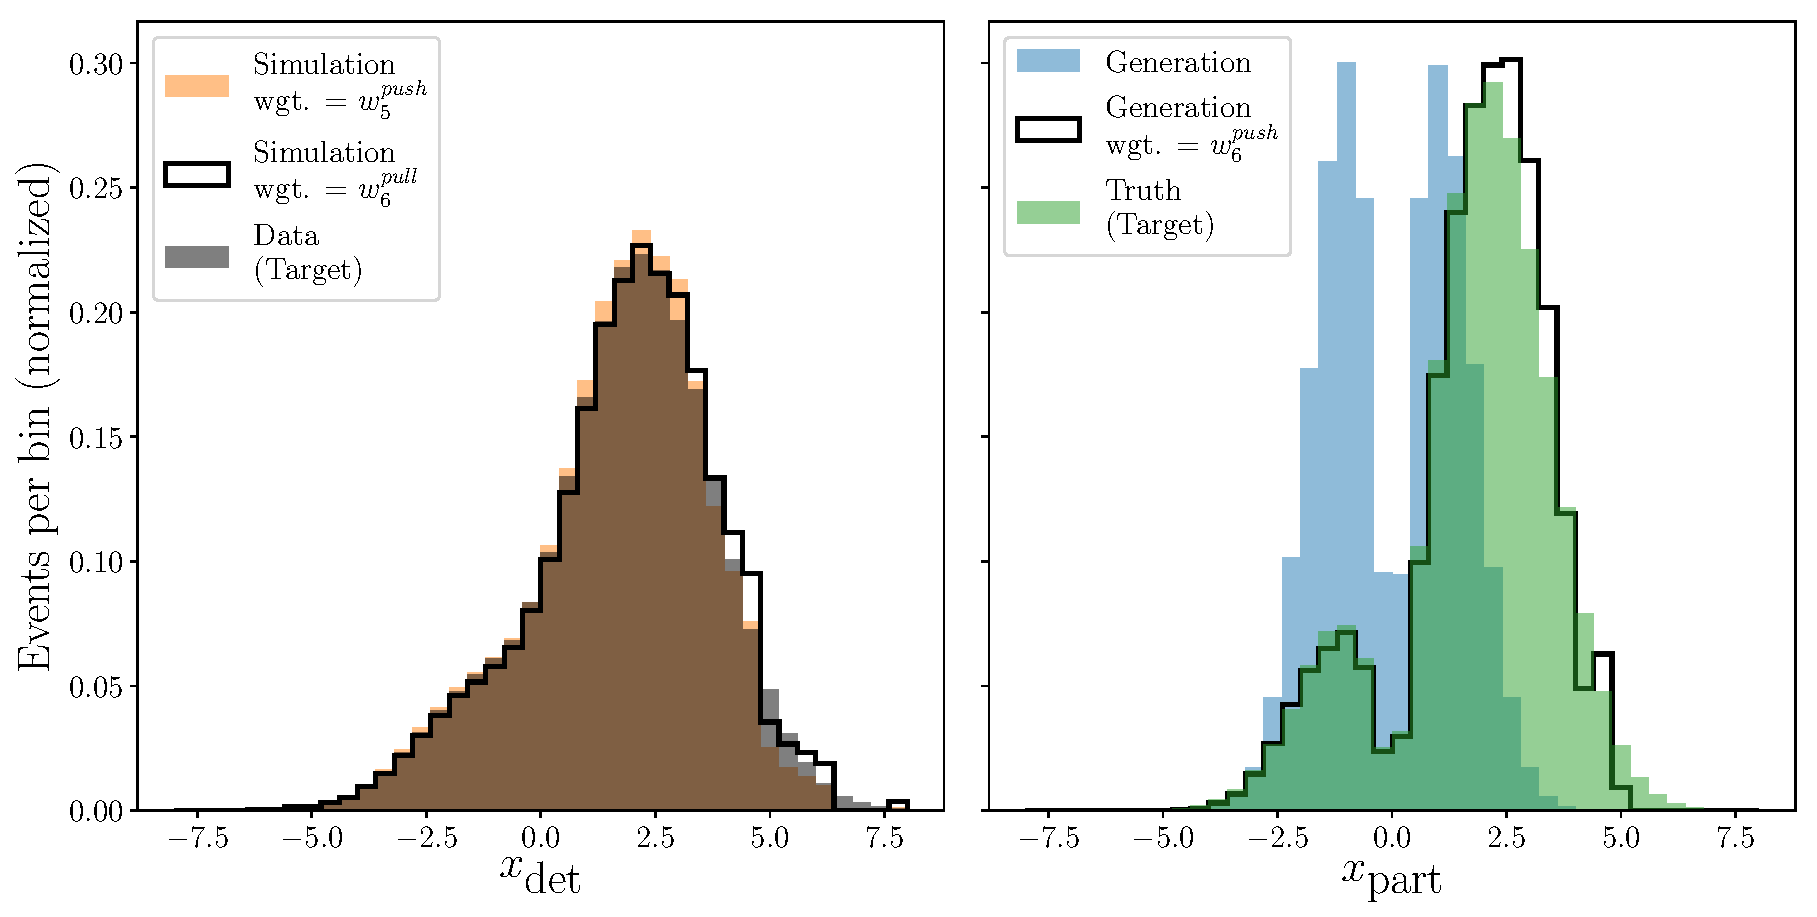
\includegraphics[width=0.45\textwidth]{Figures/GaussianToyExample/GaussianToyExample-MCUnfoldingResultsIteration06.pdf}}
\caption{An illustration of six iterations of the OmniFold algorithm to the one-dimensional Gaussian example with initial MC event weights injected.  For each iteration, the left plot is the detector-level distribution with weights $\omega_n$ and the right plot is the particle-level distribution with weights $\nu_n$.}
\label{fig:gaussian:MCiterations}
\end{figure}

\clearpage

\subsection{Event weights and normalization}
\label{sec:weights}

Each MC event $i$ is assigned a weight $w^\mathrm{MC}_i$ by the MC generator, and we further normalize this weight to the cross section times the integrated luminosity according to the standard procedure used at ATLAS to arrive at
\begin{equation}
  \label{eq:mc-norm}
  w^\mathrm{y}_i = w^\mathrm{MC}_i \frac{\mathcal{L}\,k\,\sigma_\mathrm{MC}\,\varepsilon}{\sum_i w^\mathrm{MC}_i},
\end{equation} 
where $\mathcal{L}$ is the integrated luminosity of the data and $k$, $\sigma_\mathrm{MC}$ and $\varepsilon$ are the $k$-factor, MC cross section and filter efficiency, respectively, for the MC sample in question, and the sum in the denominator runs over all generated MC events. This normalization is done for each MC sample, i.e.\ separately for the three different MC campaigns (each with different $\mathcal{L}$) and also separately for different 'slices', if applicable.

At reconstructed level, the event weight is further corrected as described in section~\ref{subsec:MCCorr}, and we get
\begin{equation}
  \label{eq:mc-norm-reco}
  w^\mathrm{reco}_i = w^\mathrm{y}_i \prod_c\,w^\mathrm{corr}_{ci},
\end{equation} 
where the product runs over the (five) different corrections, each with index $c$, namely: the pileup reweighing, the trigger efficiency SF, and the three muon efficiency SFs. When plotting any reconstructed distribution, such as the ones seen in figures~\ref{fig:MuActual}-\ref{fig:trackInfo}, we use $w^\mathrm{reco}$ to arrive at the MC predicted event yields, and similarly when plotting a truth distribution, $w^\mathrm{y}$ is used such that we get truth fiducial event yields in each bin.


At reco level, each MC event is hence represented by $(w^\mathrm{reco},\vec{x}_\mathrm{reco})$ and at truth level by $(w^\mathrm{y},\vec{x})$.
The unfolding procedure will correct the event weights of the truth events (keeping the features $\vec{x}$ the same), and we get: $(\nu(\vec{x})\,w^\mathrm{y},\vec{x})$.


We can further normalize the event weight according to:
\begin{equation}
  \label{eq:xsec-norm}
  w_{i} = \frac{\nu(\vec{x}_i)\,w^\mathrm{y}_{i}}{\mathcal{L}},
\end{equation}
where $\mathcal{L}$ is the full Run-2 integrated luminosity. The weights $w_i$ defined according to equation~\ref{eq:xsec-norm} now has units of cross section and the sum of such weights of all events that fall in any fiduciary region will constitute a measurement of the associated fiducial cross section. This can be written as:
\begin{equation}
  \label{eq:fid-xsec}
  \hat{\sigma}_{k} = \sum_{i}^{N_\mathrm{events}}w_{i}\,\mathcal{I}[b(\vec{x}_{i})=k] = \sum_{i\in B_k} w_i,
\end{equation}
where $b(\vec{x}_{i})$ returns an index $k\in\{0,1,2,...,n_\text{bins}\}$ corresponding to the fiducial region event $i$ falls in (based on its features $\vec{x}_i$), 
and $\mathcal{I}[\cdot]$ is the indicator function that is 1 when $\cdot$ is true and zero otherwise. The last equality use a more sloppy notation: the sum runs over all events $i$ that fall in bin $k$, where $B_k$ denote the set of events that fall in the bin (based on their $\vec{x}$). 
\todo{We are planning to normalize all provided events according to equation~\ref{eq:xsec-norm} such that plotting any distribution immediately results in a differential cross section.}
\clearpage


